\documentclass[hidelinks,12pt]{wzmgr}
\special{papersize=210mm,297mm}
% Wersja XeLaTeX
\usepackage{mathtools}
\usepackage[polish]{babel}
\usepackage[no-math]{fontspec}
\usepackage{xeCJK,makeidx}
\usepackage{setspace,etoolbox,csquotes,indentfirst}
\usepackage[top=2.5cm,left=2.5cm,right=2.5cm,bottom=2.5cm]{geometry}
\usepackage{url}
\usepackage[usenames,dvipsnames,svgnames,table]{xcolor}
\usepackage{blindtext}
\usepackage[inline]{enumitem}
\usepackage{xcolor}
\usepackage{graphicx}
\graphicspath{ {images/} }
\usepackage{float}
\usepackage{multirow}
\usepackage{array}
\usepackage{tabularx}
\usepackage{longtable}
%\usepackage{ltablex}
%\usepackage[hidelinks]{hyperref}


\makeatletter
\g@addto@macro{\UrlBreaks}{\UrlOrds}
\makeatother
\setmainfont[Mapping=tex-text]{Adobe Text Pro}
\setsansfont[Scale=0.88]{IPAexGothic}
\setCJKmainfont{SimSun}
\setCJKsansfont{SimHei}
\setCJKmonofont{SimHei}
\newCJKfontfamily{\ipaexgothic}{IPAexGothic}
\newCJKfontfamily{\korm}{NanumMyeongjo}
\newtoggle{brudnopis}\newtoggle{prowincjepy}
\togglefalse{brudnopis} % change \toggletrue to \togglefalse to disable comments
\toggletrue{prowincjepy}
\newcommand{\prowincja}[1]{\iftoggle{prowincjepy}{ (#1)}{}}
\newcommand{\Korean}{\korm\CJKspace}
\newcommand{\toponim}[1]{\textsf{#1}}
\newcommand{\nazwisko}[1]{#1}
\newcommand{\pinyin}[1]{\mbox{\textit{#1}}}
\newcommand{\jyutping}[1]{\mbox{\textit{#1}}}
\newcommand{\romaji}[1]{\mbox{\textit{#1}}}
\newcommand{\foreign}[1]{\textit{#1}}
\newcommand{\fnm}{\footnotemark}
\newcommand{\komentarz}[1]{\iftoggle{brudnopis}{\colorbox{Red}{#1}}}

%terminy
\newcommand{\terminprosty}[1]{\textbf{#1}}
\newcommand{\termin}[3]{\terminprosty{#1} (#2 \pinyin{#3}) --}
\newcommand{\terminpodwojny}[6]{\terminprosty{#1} (#2 \pinyin{#3}) lub
\terminprosty{#4} (#5 \pinyin{#6}) --}
\newcommand{\terminprostyzpodwojnym}[7]{\terminprosty{#1}:

\terminpodwojny{#2}{#3}{#4}{#5}{#6}{#7}}
\newcommand{\termindwapinyiny}[5]{\terminprosty{#1} (#2 \pinyin{#3} lub #4
\pinyin{#5}) --}

%deklaracje i misc czeste terminy
\newcommand{\wiatry}{wschodni, południowy, zachodni lub północny}
\newcommand{\smoki}{czerwony, zielony lub biały}
\newcommand{\hu}{\pinyin{hu} }
\newcommand{\huend}{\pinyin{hu}}
\newcommand{\hua}{\pinyin{hua}}
\newcommand{\peng}{\pinyin{peng}}
\newcommand{\gang}{\pinyin{gang}}
\newcommand{\dekchi}{\pinyin{chi}}

%deklaracje
\newcommand{\deklaracja}[1]{\pinyin{#1} -- }

%fan
\newcommand{\fan}[3]{%
  \begin{tabular}[x]{@{}c@{}}#1\\#2\\\pinyin{#3}\end{tabular}}
\newcommand{\tabsplit}[2]{%
  \begin{tabular}[x]{@{}c@{}}#1\\#2\end{tabular}}


%morozowy stuff do cytowania
%\newcommand{\defspacing}{\spacing{1.32}}
%\newcommand{\quotespacing}{\spacing{1.1}}
%\newcommand{\longquote}[1]{\quotespacing\blockquote{\itshape #1}\defspacing}

%moja obsluga cytowania
%\usepackage{quotchap}
\usepackage{epigraph}

\author{Piotr Chabelski}
\title{Madżong}
\nralbumu{XXXXX}
\kierunek{Filologia, specjalność sinologia}
\opiekun{dr Maria Kurpaska}
%\email{dmuhafc@gmail.com}
\UniversityName{Uniwersytet im. Adama Mickiewicza --- Wydział Neofilologii}
\nrwersji{0.0}
\miejsce{Poznań}
%\hyphenation{ La\.n-kā-va-tā-ra}
\makeindex
\begin{document}
\onehalfspacing
\maketitle
\introduction
% %%%%%%%%%%%%%%%%%%%%%%%%%%%%%%%%%%%%%%%%%%%
% DEFINICJA OBOWIĄZUJĄCA W PRACY
% %%%%%%%%%%%%%%%%%%%%%%%%%%%%%%%%%%%%%%%%%%%%%
%\mahjongdef % oddzielna sekcja w spisie treści (,,drugi wstęp'')
\def \traditionalstonesfootnote {\getrefnumber{definicja_tradycyjne}} %zmienna do referencji
% przypisu przy kamieniach zapisanych w znakach tradycyjnych
\subsection{Definicja przyjęta na potrzeby niniejszej pracy}
\label{definicja}
Madżong to gra spełniająca %definicję opisaną w sekcji 1.1.1 niniejszej pracy
% oraz
następujące warunki:

% %%%%%%%%%%%%%%%% WARUNEK A
\begin{enumerate}[label={\alph*)}] \item Gra wykorzystuje zestaw składający się
z kamieni, które kształtem przypominają płytki domina, jednakże są nieco grubsze
i krótsze. Dopuszczalna jest także możliwość wykorzystywania kart zamiast
kamieni.
% %%%%%%%%%%%%%%%% WARUNEK B
\item Kamienie (lub karty) mają grawerowane lub malowane oznaczenia,
przyporządkowujące je do odpowiednich grup figur lub talii. Zestaw uwzględnia
następujące talie i figury\footnote{Skład zestawu do gry został opisany w tej
sekcji uwzględniając wszystkie dopuszczalne jego możliwości.
Precyzyjny opis współczesnego zestawu do gry w madżonga zgodny z
międzynarodowymi zasadami turniejowymi znajduje się  na stronie
\pageref{guobiao_zestaw}.}:
	\begin{itemize}
	  \item 3 talie (kółka (筒 \pinyin{tǒng} lub 饼 \pinyin{bǐng}), bambusy (索
	  \pinyin{suǒ}) oraz liczby (万 \pinyin{wàn})) z kamieniami o
wartościach od 1 do 9; dopuszczalna jest także talia rang zamiast talii liczby
(oznaczana przez znaki 卐 (\pinyin{wàn}, dla kamienia o wartości 1) oraz 品 
(\pinyin{pǐn}, dla kamieni o wartościach od 2 do 9)); 
\item 4 wiatry \label{wiatry}
(wschód(東\footnote{\label{definicja_tradycyjne}Znaki wyjątkowo zapisane w formie
tradycyjnej, jako że w takiej występują na kamieniach. Dla znaku 東  forma
uproszczona to 东, dla 將 jest to 将, dla 發 -- 发, dla 龍 -- 龙, a dla 鳳 -- 凤.}
\pinyin{dōng}), południe (南 \pinyin{nán}), zachód (西 \pinyin{xī}) i północ (北
\pinyin{běi}));  dopuszczalny jest także wariant, w którym zamiast 4 wiatrów
występuje 4 możnych (diuk (公 \pinyin{gōng}),  markiz (侯 \pinyin{hóu}),  generał
(將\footnotemark[\traditionalstonesfootnote] \pinyin{jiàng}) oraz minister (相
\pinyin{xiàng}));
	  \item 3 smoki (biały (白 \pinyin{bái}), zielony
	  (發\footnotemark[\traditionalstonesfootnote] \pinyin{fā}) i czerwony (中
	  \pinyin{zhòng})); dopuszczalny jest także wariant, w którym zamiast smoka
	  zielonego jest smok bez przydzielonej mu barwy\footnote{,,3 Smoki'' w
	  kolorach białym, zielonym i czerwonym to zasadniczo termin zachodni, nie
	  chiński.
	  Chińczycy używają określenia ,,3 \pinyin{yuan}'' (三元牌 \pinyin{sān yuán
	  pái}). We wczesnych zestawach do gry w madżonga występował jednakże
	  kamień oznaczany znakiem smoka --
	  龍\footnotemark[\traditionalstonesfootnote].}
	  (龍\footnotemark[\traditionalstonesfootnote] \pinyin{lóng}), a zamiast smoka
	  czerwonego -- feniks
	  (鳳\footnotemark[\traditionalstonesfootnote]\pinyin{fèng});
	  \item opcjonalnie kwiaty i/lub pory roku w różnej ilości;
	  \item opcjonalnie dżoker lub inne kamienie specjalne.
	\end{itemize}
%%%%%%%%%%%%%%%%%
% WARUNEK C
\item Kamienie o odpowiednich oznaczeniach występują w obrębie jednego zestawu
do gry w następujących ilościach:
	\begin{itemize}
	  \item 4 egzemplarze każdego z kamieni o numerach od 1 do 9 w każdej z 3 talii
	  (łącznie 108 kamieni);
	  \item 4 egzemplarze każdego z kamieni wiatrów (łącznie 16 kamieni);
	  \item 4 egzemplarze kamieni każdego z 3 smoków (łącznie 12 kamieni);
	  \item łączna liczba kamieni kwiatów i pór roku może się wahać od 0 do ponad
	  20;
	  \item łączna liczba kamieni specjalnych oraz dżokerów może się wahać od
	0 do ponad 20.
	\end{itemize} 
%%%%%%%%%%%%%%%%%
% WARUNEK D
\item Zasady gry uwzględniają następujące punkty:
	\begin{itemize}
	  \item gra polega na kompletowaniu przez graczy określonego przez zasady
	  układu kamieni zwanego dalej ,,ręką''\footnote{\label{reka}W niektórych
	  kontekstach termin ,,ręka'' może oznaczać również pełne jedno rozdanie w czasie gry (盘
	  \pinyin{pán}) (Shìjiè Májiàng Zǔzhī 2014). Aby uniknąć niejednoznaczności,
	  na potrzeby niniejszej pracy termin ten nie będzie używany w tym znaczeniu.}
	  (手牌 \pinyin{shǒupái});
	  \item gracz, który skompletuje gotową rękę jako pierwszy, wygrywa rozdanie;
	  \item choć liczba kamieni tworzących rękę może ulec zmianie w zależności od
	  wariantu gry, musi się ona składać z pewnej liczby ,,grup'' (pomniejszych
	  układów składających się z od 3 kamieni\footnote{Spotykane są również grupy
	  składające się z 4 lub 5 kamieni, jednakże wymagają one specjalnych
	  deklaracji w czasie gry oraz dobrania dodatkowych kamieni na wymianę. W
	  rezultacie, potencjalny czwarty lub piąty kamień w grupie nie wpływa na
	  budowę ręki, lecz na późniejsza punktację, stąd są one dalej traktowane
	  jako kamienie bonusowe.}) oraz dokładnie jednej pary (2 kamieni tego samego
	  typu), zgodnie z poniższym wzorem:
	  \begin{equation*}
	  n = 3g + 2 + x
	  \end{equation*}
	  gdzie n to liczba kamieni tworzących rękę, g to liczba grup, a x to liczba
	  kamieni bonusowych\footnote{Kamienie bonusowe nie zawsze są traktowane jako
	  część ręki gracza, jednakże są z nią ściśle powiązane, w związku z czym
	  autor pracy uznał za stosowne uwzględnić je we wzorze.} (kwiatów lub
	  rozszerzeń grup do 4 lub 5 kamieni);
	  \item gra jest skierowana do 4 graczy (opcjonalnie zasady mogą
	  zezwalać na grę dla 3 graczy).
	\end{itemize} 
\end{enumerate}
(Sloper 2006; Stanwick \& Xu; Shìjiè Májiàng Zǔzhī 2006)
\chapter{Historia madżonga}
% %%%%%%%%%%%%%%%%%%%%%%%%%%%%%%%%%%%%%%%%%%%%%%%%%%%%%%%%%%%%%%%%%%%%%%%%
% POCZĄTKI
% %%%%%%%%%%%%%%%%%%%%%%%%%%%%%%%%%%%%%%%%%%%%%%%%%%%%%%%%%%%%%%%%%%%%%%%%
\section{Początki madżonga}
% %%%%%%%%%%%%%%%%%%%%%%%%%%%%%%%%%%%%%%%%%%%%
% L.L. HARR
% %%%%%%%%%%%%%%%%%%%%%%%%%%%%%%%%%%%%%%%%%%%%%
\subsection{Mity na temat starożytnych początków madżonga}
Nie jest kwestią prostą ustalenie od którego momentu w historii możemy mówić o
madżongu. Sprawa ta jest tym trudniejsza, że wiele powszechnie dostępnych źródeł
zawiera informacje nieprecyzyjne lub wręcz całkowicie błędne. 

Niezwykle popularnym, choć niewiele mającym wspólnego z rzeczywistością, jest
pogląd, że madżong jest grą niezwykle starą, pamiętającą czasy Konfucjusza,
czyli V wiek przed naszą erą. Ów pogląd wywodzi się z niesławnej publikacji Lew
Lysle Harra wydanej w 1922 roku pod tytułem ,,Pung Chow''\footnote{Tytuł książki
L.L. Harra ,,Pung Chow'' to jedna z popularniejszych nazw, jaką określano
madżonga w pierwszej połowie XX wieku. ,,Pung'' i ,,chow'' to przyjęty przez
Harra zapis 2 spośród najpopularniejszych ruchów dozwolonych w madżongu --
współcześnie są one znane jako \pinyin{peng} (碰 pèng) i \pinyin{chi} (吃 chī).}
(Harr 2008).
Lew Lysle Harr był w Chinach w 1919 roku reprezentantem amerykańskiej firmy
Graton and Knight Belting Company. Uznał on, że masowo produkowane zestawy do
madżonga w zunifikowanej, jednolitej formie pozwoliłoby na łatwą wymianę
zgubionych kamieni oraz byłyby łatwiejsze do sprzedaży.
Wyżej wymieniona publikacja to spisany przez niego podręcznik do nauki zasad
gry, który w swoim wstępie zawiera notatkę o historii i pochodzeniu madżonga.
Według jej treści, madżong w swojej pierwotnej postaci wymyślony został około
472 roku przed naszą erą na dworze króla państwa Wu, czyli w okolicach
współczesnego Ningbo\footnote{Ningbo (宁波 \pinyin{Níngbō}) - miasto we
wschodnich Chinach, w prowincji Zhejiang (浙江 \pinyin{Zhèjiāng}), port handlowy i
rybacki nad Morzem Wschodniochińskim.}. Madżong miał tam funkcjonować pod nazwą
\textit{Pe-Ling} jako gra umilająca czas samemu królowi, jego rodzinie i
bliskiemu otoczeniu. Karą za spędzanie w ten sposób czasu przez niższe warstwy
społeczeństwa była śmierć poprzez ścięcie głowy. Później dostęp do gry miał
zostać rozszerzony do kasty kupców, a dopiero w połowie XIX wieku naszej ery
stać się powszechnie dostępnym.
Publikacja prezentująca powyższe informacje miała służyć reklamie produktu,
który L.L. Harr zamierzał sprzedawać. Jako że zgodnie z ówczesnymi (jak
też i współczesnymi) badaniami nad pochodzeniem madżonga, gra nie istniała przed
XIX wiekiem naszej ery, a cała historia podana we wstępie do ,,Pung Chow'' była
nieprawdziwa, książka spotkała się z ostrą krytyką, a firma Harra zbankrutowała
w 1925 roku. Jednakże, choć L.L. Harr nie odniósł sukcesu w dziedzinie sprzedaży
madżonga, jego książka jest współcześnie powszechnie dostępna w księgarniach, a
ostra krytyka, z jaką się spotkała zaraz po jej pierwszej publikacji nie jest
wiedzą powszechną. W wyniku tego, że Harr faktycznie znajdował się w Chinach w
latach dwudziestych XX wieku, gdy madżong po raz pierwszy zaczął trafiać do
szerokiej publiczności w Europie i Ameryce Północnej, wiele źródeł uznaje jego
książkę za wiarygodną i odnosi się do zawartych w niej fałszywych informacji
(Greenfield 2010; Harr 2008; Mah Jong Museum).
% %%%%%%%%%%%%%%%%%%%%%%%%%%%%%%%%%%%%%%%%%%%%
% FAKTYCZNE POCZĄTKI
% %%%%%%%%%%%%%%%%%%%%%%%%%%%%%%%%%%%%%%%%%%%%%
\subsection{Gry karciane - rzeczywiste początki madżonga}
Nawet po eliminacji źródeł zawierających informacje niewątpliwie fałszywe,
ustalenie dokładnego momentu pojawienia się madżonga po raz pierwszy pozostaje
kwestią trudną. Częścią problemu jest fakt, że już wtedy, gdy pierwszy raz
zaczęto używać nazwy ,,madżong'', nie była to gra całkowicie nowa, lecz raczej
kombinacja zasad szeregu funkcjonujących na terenie Chin w XIX wieku i wcześniej
hazardowych gier karcianych. 

%dopisany fragment podpierający to, ze w Chinach o hazardzie pisać było wstyd
%i stąd jest mało chińskich źródeł
Sprawa okazuje się być tym bardziej skomplikowana w związku z długą historią
uprawiania hazardu, który był w Chinach popularny już od czasów starożytnych.
Pierwsze odnotowane przypadki jego uprawiania sięgają końca dynastii Zhou (周
Zhōu) (między 800 a 256 rokiem przed naszą erą), jednakże niektórzy historycy
sugerują, że faktycznie do pierwszych takich zajść mogło dochodzić już za
dynastii Shang (商 Shāng)(między 1700 a 1027 rokiem przed naszą erą), a nawet Xia
(夏 Xià) (między 2000 a 1500 rokiem przed naszą erą). Od tego czasu chińscy
władcy wielokrotnie próbowali kontrolować te zjawiska, a nawet całkowicie
zakazywać hazardu, jednakże nie były to rozwiązania trwałe aż do całkowitego
zakazu wprowadzonego w roku 1949. Przykładowo, choć Zhu Yuanzhang (朱元璋 Zhū
Yuánzhāng), pierwszy cesarz dynastii Ming (明 Míng) w latach 1368-1398, zakazał
hazardu na początku swoich rządów, sam nie przestrzegał własnego rozporządzenia,
grając często na pieniądze ze swoimi współpracownikami (Tse, Samson \& Yu, Alex
C.H. \& Rossen, Fiona \& Wang, Chong-Wen 2010).

Mimo że przez tysiące lat hazard pozostawał popularnym sposobem spędzania czasu
dla wszystkich warstw społeczeństwa, nie był on w żadnym razie powodem do dumy.
Jedno z chińskich źródeł traktujących o hazardzie pochodzące z 1783 roku, do
których odnosi się niniejsza praca, zostało zatytułowane ,,Plotki o
Świniopasach'' (牧猪闲话 \pinyin{Mùzhū Xiánhuà}), co zwraca uwagę na to, w jaki
sposób jego autor, Jin Xueshi (金学诗 Jīn Xuéshī), traktował ten temat.  W czasie,
gdy starsze gry karciane powoli przekształcały się w grę nazywaną ,,madżongiem''
wzbudzało to w większym stopniu zainteresowanie naukowców napływających z
Ameryki Północnej i Europy, niż tych pochodzących z Chin. Jako że pierwsi uczeni
publikujący na ten temat w drugiej połowie XIX wieku nie zajmowali się
ustaleniem historycznych początków madżonga, lecz raczej próbowali przedstawić
społeczeństwu zachodniemu, wiele dat podawanych przez autora w dalszej części
tego rozdziału jest jedynie przybliżeniem na podstawie powstałych dużo później
rekonstrukcji.

% %%%%%%%%%%%%%%%% GRY KARCIANE
Jednakże, przed ustaleniem momentu pojawienia się madżonga należy poświęcić
uwagę również grom karcianym, z których prawdopodobnie się on wywodzi.

% %%%%%%%%%%%%%%%% SHIHU
Jedną z nich, która uznawana jest za spokrewnioną z madżongiem, jest
\pinyin{shihu} (十壶 \pinyin{shíhú}). Nazwę możnaby dosłownie przetłumaczyć jako
,,10 dzbanków'', choć spotykane jest także tłumaczenie ,,10 punktów'' (Stanwick,
Xu za Lo 2004). Można zatem przypuścić, że nazwę gry można również zapisać 十和
(\pinyin{shíhú}\footnote{Choć najczęstsze czytanie znaku 和 to ,,\pinyin{hé}'', a
znak ten najczęściej oznacza pokój, harmonię, a także występuje w zdaniu jako
spójnik, w kontekscie madżonga i wielu spokrewnionych z nim gier czytany jest on
,,\pinyin{hú}''. Oznacza on wówczas skompletowanie ręki, czyli zwycięstwo w
rozdaniu. Analogicznie, prawdopodobnie najcelniejszym tłumaczeniem \pinyin{mohu}
(patrz: strona \pageref{mohu_page}) jest ,,kompletowanie ręki w milczeniu''.}),
czyli dosłownie ,,10 wygranych''. Do gry służył zestaw kart papierowych, których liczba zazwyczaj wynosiła 120, choć
można było również spotkać warianty na 125, 132, a nawet 160 kart. Zestaw
składał się z:
\begin{itemize}
  \item 36 kart (4 egzemplarze każdego rodzaju karty) w każdej z 3 talii (餅
  \pinyin{bǐng}, 索 \pinyin{suǒ} oraz 万 \pinyin{wàn}), łącznie 108 kart;
  \item po 4 egzemplarze 3 kart kwiatów (花 \pinyin{huā}), łącznie 12 kart;
  \item rzadziej innych dodatkowych kart.
\end{itemize}
Jak łatwo zauważyć, choć skład takiego zestawu nie spełnia norm przyjętych w
madżongu, jest do nich bardzo zbliżony. Oznaczenia na kartach również odbiegają
od tych stosowanych w madżongu (Rysunek 1.1). Sama gra w \pinyin{shihu},
podobnie jak gra w madżonga, polegała na ułożeniu określonego układu w procesie
dobierania i odrzucania kart przez graczy po kolei. Zwycięski układ musiał być
wart minimum 10 punktów. \pinyin{Shihu} niewątpliwie zostało wymyślone przed
madżongiem, jako że jest wspominane w dziele pochodzącym z 1796 roku --
,,Malowane Łodzie Przyjemności z Yangzhou''\footnote{Tytułowe ,,łodzie
przyjemności'' to domy publiczne w Yangzhou (扬州 \pinyin{Yángzhōu}), mieście we
wschodnich Chinach. Klienci owych domów publicznych grywali w \pinyin{shihu},
nie jest jednakże jasnym, czy była to usługa świadczona przez same instytucje,
czy też zwyczajnie popularna w ich gronie rozrywka (Stanwick \& Xu).}
autorstwa \pinyin{Li Dou} (李斗, \pinyin{Lǐ Dǒu}) (Stanwick \& Xu).

\begin{figure}[h]
\centering
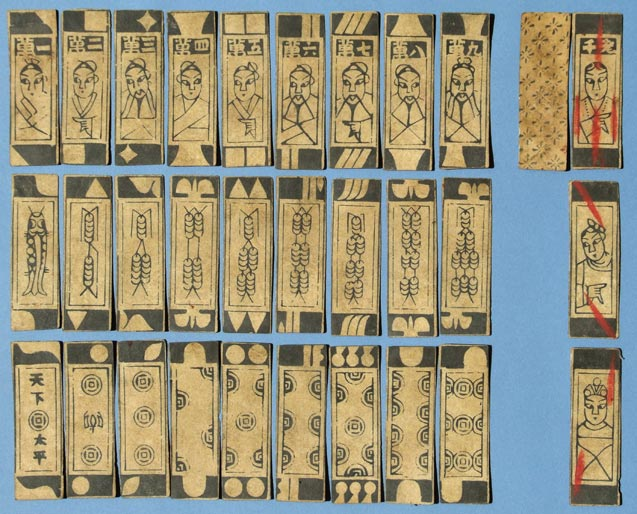
\includegraphics[width=0.75\textwidth]{1_shihu.jpg}
\caption{Niekompletny zestaw do gry w \pinyin{shihu}; 30 spośród 120 kart;
Chiny, ok. 1900 r;  źródło:
http://www.themahjongtileset.co.uk/tile-set-history/earliest-suit-names/}
\end{figure}

% MADIAO
Same karty używane do gry w \pinyin{shihu} wykorzystywane były również do wielu
innych gier, a ich wcześniejszym zastosowaniem prawdopodobnie była gra w
\pinyin{madiao} (馬吊 \pinyin{mǎdiào}), czyli dosłownie ,,wieszanie konia'',
pochodząca z czasu rządów cesarza Kangxi (康熙 Kāngxī), czyli z lat 1661--1722.
(Jin 1783) Zestaw \pinyin{madiao} składał się z 40 kart w 4 taliach -- czwarta
talia, niewystępująca w grach wywodzących się z \pinyin{madiao}, nazywana była
,,dziesiątkami myriad'' (万贯 \pinyin{wànguàn}). Później wykorzystywano zestawy
zawierające tylko 3 talie (czyli 30 kart) do innych gier (Stanwick \& Xu).

%MOHU
\label{mohu_page}
Przykładem innej gry wykorzystującej zestaw do \pinyin{madiao} jest
\pinyin{mohu} (默和 \pinyin{mòhú}). Gra była przeznaczona dla			
% tu było tłumaczenie, czym jest mohu, ale zostało przy shihu kawałek wcześniej
4 graczy i wymagała 60 kart (czyli najprawdopodobniej 2 zestawów kart
\pinyin{madiao} pozbawionych talii dziesiątków myriad). Jeden z graczy rozdawał
wszystkim uczestnikom po kolei po 1 karcie, aż każdy miał ich po 10. Następnie
gracze układali je w ciszy. Dalsza rozgrywka polegała na dobieraniu kart z
pozostałych 20 w celu ułożenia zwycięskiego układu (jeden z graczy, ale nie ten
odpowiadający za pierwsze rozdanie kart, rozdawał kolejne) (Jin 1783; Stanwick
\& Xu).
% 
% \footnote{,,Natrafianie na układ z
% kart'' to dosłowne znaczenie nazwy \pinyin{penghu}, jednakże prawdopodobnie jej
% pochodzenie jest nieco inne. \pinyin{Peng} (碰 \pinyin{pèng}) to jedna z
% najczęściej stosowanych deklaracji we współczesnym madżongu. Jej użycie pozwala
% na dobranie kamienia odrzuconego przez innego gracza do własnej trójki takich
% samych kamieni. Prawdopodobnie zachodzi związek pomiędzy tą nazwą, a nazwą gry w \pinyin{penghu}.}


% PENGHU
Inną tego typu grą jest \pinyin{penghu} (碰和 \pinyin{pènghú} -- dosłownie
,,natrafianie na układ z kart'').
W \pinyin{penghu} grano 4 lub 5 zestawami do \pinyin{madiao}, czyli łącznie 120
lub 150 kartami (Stanwick \& Xu). Inne źródło sugeruje, że stosowano 2 lub 2,5
zestawu do \pinyin{mohu} (Jin 1783), co sumuje się do tej samej liczby kart.
Nie jest oczywistym, czy gra wykształciła się bezpośrednio z \pinyin{madiao},
czy też pośrednio z \pinyin{mohu} (jak sugeruje Jin 1783).
Pojawiają się w niej układy występujące również we współczesnym madżongu, jak na
przykład \pinyin{peng}\footnote{\pinyin{peng} (碰 \pinyin{pèng}) to jedna z
 najczęściej stosowanych deklaracji we współczesnym madżongu. Jej użycie pozwala
 na dobranie kamienia odrzuconego przez innego gracza do własnej trójki takich
 samych kamieni. Występuje również w grze w \pinyin{penghu} i jest elementem jej
 nazwy.}. Można sądzić, że niektóre źródła mowiące tylko o \pinyin{shihu} lub
 tylko o \pinyin{penghu} nie rozróżniały tych dwóch gier, jako że ich zasady i
 skład zestawów do gry były do siebie zbliżone (Jin 1783; Stanwick \& Xu).

% PODSUMOWANIE KART
Karty do \pinyin{madiao} były również wykorzystywane do szeregu innych,
pomniejszych gier, jak \pinyin{kanhu} (看虎 \pinyin{kànhǔ} \label{kanhu}--
,,obserwowanie tygrysa''), \pinyin{hunjiang} (混江 \pinyin{hùnjiāng} -- ,,zwijanie rzeki'') oraz
\pinyin{suohu} (梭和 \pinyin{suōhú} - ,,układanie kart ruchem w tę i z
powrotem'') (Stanwick \& Xu). Każda z nich jest warta wspomnienia, jako że wielu
pasjonatów oraz badaczy na przełomie XIX i XX wieku określało własne zestawy do
madżonga właśnie ich nazwami (nie będąc jeszcze świadomym różnicy).
Można wręcz przypuszczać, że funkcjonowały one przez długi czas równolegle z
nowo wykształconym madżongiem, a być może nawet grano w nie przy pomocy
kamieni zamiast kart.
% %%%%%%%%%%%%%%%%%%%%%%%%%%%%%%%%%%%%%%%%%%%%
% MADŻONG NA PRZEŁOMIE XIX/XX WIEKU
% %%%%%%%%%%%%%%%%%%%%%%%%%%%%%%%%%%%%%%%%%%%%%
\subsection{Madżong pod koniec XIX wieku}
Ciężko określić, w którym dokładnie momencie zaczęto używać kamieni do gry
zamiast kart\footnote{Ze względu na nierozróżnianie ich w języku i określanie
wspólnym mianem \pinyin{pai}, zgodnie z zapisem w sekcji 1.1.2.}, jednakże było
to już niewątpliwie praktykowane w latach siedemdziesiątych XIX wieku (Stanwick
2004). Niemiecki tłumacz Carl Himly w latach 1868-1876 zdobył zestaw bambusowych
kamieni, które w swoich publikacjach z 1889 i 1901 określał jako ,,bambusowe
\pinyin{pai} z Ningbo\footnote{Ningbo (宁波 \pinyin{Níngbō}) -- miasto we
wschodnich Chinach, w prowincji Zhejiang (浙江 Zhèjiāng), port handlowy i rybacki
nad Morzem Wschodniochińskim.}'' (宁波竹牌 \pinyin{Níngbō zhúpái}). Nie spełnia on
definicji madżonga przyjętej na potrzeby tej pracy (brakuje w nim kamieni
czerwonego oraz zielonego smoka), jednakże jest do niej bardzo zbliżony.
(Stanwick, Xu za Himly 1889-1901) Bardzo podobne zestawy (w których uwzględniony
już został smok czerwony, jednakże wciąż brakowało zielonego) pochodzące z
okresu pomiędzy 1869 a 1875 rokiem zostały dostarczone przez George'a B.
Glovera\footnote{George B. Glover, wicekonsul Stanów Zjednoczonych w Szanghaju w
latach 1858-1859. Później w latach od 1859 do około 1882 komisarz urzędu celnego
w różnych miejscach w Chinach (Wikipedia 2013).} do Amerykańskiego Muzeum
Historii Naturalnej (American Museum of Natural History) (Stanwick 2004). Glover
napisał w 1875 roku notatkę, która została załączona do owych zestawów, w której
prawdopodobnie po raz pierwszy użyto poza Chinami nazwy
,,wróbel''\footnote{Glover w 1975 roku użył nazwy \pinyin{jiaqiao} (家雀
\pinyin{jiāqiǎo}), czyli dosłownie ,,wróbel domowy''. Współcześnie łatwiej można
spotkać określenie \pinyin{maque} (麻雀 \pinyin{máquè}), które również oznacza
wróbla, jednakże regionalnie można wciąż spotkać się także z użyciem tego słowa
jako synonim madżonga. W języku japońskim \pinyin{majian}, które zapisywane jest
tymi samymi znakami, co \pinyin{maque} po chińsku, również oznacza madżonga
(Stanwick \& Xu).}, która współcześnie jest jednym z wielu synonimów madżonga.
Zestawy różniły się pomiędzy sobą składem, jednakże można przyjąć że służyły do
tych samych lub spokrewnionych ze sobą gier. Jako że pochodziły z różnych
obszarów Chin -- Ningbo i Szanghaju, można przyjąć że stosowanie zestawów
kamieni zamiast kart stawało się w tym czasie coraz bardziej popularne w
Chinach.

Bardziej precyzyjne badania nad madżongiem rozpoczynają się w roku 1893, kiedy
to William Henry Wilkinson, pracownik konsulatu brytyjskiego w Chinach, wysłał
zbiór gier zakupionych w Chinach do profesora Stewarta Culina,\footnote{Stewart
Culin, amerykański etnograf, pracownik Uniwersytetu Pensylwanii, badacz gier,
ubioru i sztuki chińskiej; jeden z pierwszych badaczy madżonga (Wikipedia
2016).} który Culin później wystawił na wystawie World's Colombian Exposition w
Chicago. W owym zbiorze znajdowała się gra karciana, którą Wilkinson określał
jako \pinyin{khanhoo}, czyli najprawdopodobniej wspomniane na stronie
\pageref{kanhu} \pinyin{kanhu} (看虎 \pinyin{kànhǔ} -- ,,obserwowanie tygrysa'').
\pinyin{Khanhoo}, pośród innych gier wymienianych przez Wilkinsona, należało do
podzbioru określanego przez niego mianem ,,wróbli'', czyli \pinyin{maque}. Culin
zajął się badaniami na ten temat i w późniejszych publikacjach uznał ,,wróble''
Wilkinsona za przodków madżonga (Culin 1924; Greenfield 2010).

% %%%%%%%%%%%%%%%%%%%%%%%%%%%%%%%%%%%%%%%%%%%%
% XX WIEK
% %%%%%%%%%%%%%%%%%%%%%%%%%%%%%%%%%%%%%%%%%%%%%
\section{Madżong w XX wieku}

% %%%%%%%%%%%%%%%%%%%%%%%
% SZANGHAJ 20s
% %%%%%%%%%%%%%%%%%%%%%%%
\subsection{Madżong w Szanghaju lat dwudziestych XX wieku}
Jakkolwiek \pinyin{khanhoo} cieszyło się zainteresowaniem naukowców, poza
terenem Chin nie zdobyło popularności. Przełomowy moment w historii madżonga nastąpił wtedy,
gdy gra trafiła do Szanghaju. Choć zasady sformułowane zostały w Ningbo, to
Szanghaj pozwolił im się w pełni rozwinąć i trafić do szerszego grona odbiorców.
W wyniku traktatów podpisanych po zakończeniu dziewiętnastowiecznych Wojen
opiumowych\footnote{Wojny opiumowe – wspólne określenie na mające miejsce w
dziewiętnastym wieku 2 konflikty zbrojne Chin z Wielką Brytanią i Francją;
jednym z ich skutków był szereg upokarzających dla Chin traktatów wymuszających
ustępstwa handlowe przy handlu wieloma towarami, przede wszystkim opium.}, port
w Szanghaju stanowił jedną ze specjalnie wyznaczonych stref, gdzie przybysze ze
Stanów Zjednoczonych, Wielkiej Brytanii i innych państw zachodnich mogły
dokonywać swobodnej wymiany kulturowej, niepodlegając chińskiemu prawu oraz
podatkom (Greenfield 2010).

Sam Culin w 1909 roku w Szanghaju kupił „zestaw
domina wykonany z kości słoniowej”, który już spełniał definicję madżonga
opisaną na stronie \pageref{definicja}. Możemy przyjąć, że wówczas podobne
zestawy nie miały jeszcze ustalonego składu, jako że według informatora nazwiskiem Dzau Sing
Chung z Szanghaju, na którego powołuje się Culin, były one
zazwyczaj wykonywane na zamówienie, zgodnie z potrzebami klienta (Culin 1924).

Jednakże, dopóki zestaw do gry nie miał ustalonego składu i był wykonywany na
zamówienie, jego dystrybucja pozostawała problematyczna, w związku z czym szereg
osób dokonywało prób jego standaryzacji. Jedną z takich osób był Joseph A.
Babcock, reprezentant amerykańskiej firmy Standard Oil Company, który właśnie w
Szanghaju nauczył się grać w madżonga, by później
stać się najważniejszą osobą w historii popularyzacji tej gry na świecie. W
1920 roku wydał on pierwsze zasady gry w języku
angielskim, czyli ,,Czerwoną Księgę Zasad'' (\textit{Red Book of Rules}).
Książkę sprzedawano razem z zestawami do gry, którą początkowo importowano z
Chin, a później także wykonywano w Stanach Zjednoczonych. Babcock opatentował
nazwę ,,Mah-Jongg'', której różne pisownie (,,mahjong'', ,,majong'' i im
podobne) stały się powszechnie używaną na zachodzie nazwą gry. Określenie
,,madżong'', przyjęte na potrzeby niniejszej pracy, również jest jej
spolszczeniem. Wielu próbowało imitować sukces Babcocka, jednakże było
zmuszonych używać innych nazw gry, między innymi przez co nie odnieśli
porównywalnego sukcesu\footnote{Dla przykładu, wspomniany w sekcji 1.2.1 Lew
Lysle Harr był zmuszony używać nazwy ,,Pung Chow''.} (Greenfield 2010).

\subsection{Odrodzenie madżonga}
Jako że madżong w swojej pierwotnej postaci był grą hazardową, kojarzącą się z
rozwiązłym stylem życia zepsutego zachodu, został on zakazany w 1966 roku na
początku rewolucji kulturalnej\footnote{Wielka proletariacka rewolucja
kulturalna – mający miejsce w latach 1966-1976 ruch społeczno-polityczny
zapoczątkowany przez przywódcę Partii Komunistycznej Chin, Mao Zedonga.}, wraz z
wszystkimi innymi przejawami hazardu na terenie całego kraju
(Carlisle 2009).

Stworzono nowe zasady, które miały wyeliminować elementy gry hazardowej i
uzyskać grę, w której najważniejsze byłyby umiejętności gracza. Tym samym, w
1998 roku opublikowano ,,Międzynarodowy Standard Madżonga'' (国际标准麻将
\pinyin{guójì biāozhǔn májiàng}), czyli zasady międzynarodowe (w poszechnym użytku jest skrót
-- 国标麻将 \pinyin{guóbiāo májiàng}), a zakaz gry został zniesiony. W tym samym
roku madżong został w Chinach oficjalnie uznany za dyscyplinę sportową
(Carlisle 2009; Zi 2015).

W 2002 roku w Tokio odbyły się pierwsze na świecie międzynarodowe zawody w grze
w madżonga, na których obowiązywały już zasady \pinyin{guóbiāo májiàng}.
Pierwotnie miały się one odbyć w Ningbo. Zwyciężył w nich reprezentant Japonii,
Mai Hatsune (Kanazawa 2010, Nihon kenkō asa shō kyōkai kōshiki saito 2002).

W październiku 2005 roku w Pekinie utworzono Światową Organizację Madżonga
(World Mahjong Organization lub 世界麻将组织 \pinyin{Shìjiè Májiàng Zǔzhī}).
Poza Chinami, do krajów założycielskich należały między innymi Japonia, Stany
Zjednoczone Ameryki Północnej, Niemcy, Francja, Dania, Holandia oraz Węgry
(Shìjiè Májiàng Zǔzhī 2006).

W listopadzie 2007 roku w Chengdu\footnote{成都 (\pinyin{Chéngdū}) -- stolica
prowincji 四川 (\pinyin{Sìchuān}), miasto w południowo-wschodnich Chinach.} odbyły
się pierwsze oficjalne Światowe Mistrzostwa Madżonga. Od tego czasu stało się to
regularnym wydarzeniem - kolejne miały miejsce w 2010 roku w
Utrecht\footnote{Utrecht --  miasto w środkowej Holandii.} oraz w 2012 w
Chongqing\footnote{重庆 (\pinyin{Chóngqìng}) -- miasto w środkowych Chinach, jedno
z czterech miast wydzielonych Chińskiej Republiki Ludowej.} (Kǒuzhuāng Bāshì
2014).






 















\chapter{Międzynarodowe zasady turniejowe}
\label{guobiao}
\section{Opis ogólny}
Po wprowadzeniu prawa zakazującego uprawiania hazardu w Chinach w roku 1966
(patrz: strona \pageref{zakaz_1966}), gra w madżonga stała się na powrót legalna
dopiero w 1998 wraz z wprowadzeniem międzynarodowych zasad turniejowych (国标麻将
\pinyin{guóbiāo májiàng} -- patrz: strona \pageref{relegalizacja}).

Autor podjął decyzję o szczegółowym wyjaśnieniu właśnie tych zasad ze względu na
to, że to zgodnie z nimi od 2002 roku rozgrywane są ogólnoświatowe mistrzostwa
gry w madżonga (patrz: strona \pageref{pierwsze_mistrzostwa}).

Treść zasad opisana w dalszej części podrozdziału powstała na podstawie
dokumentu opublikowanego przez Światową Organizację Madżonga (patrz: strona
\pageref{wmo}) 2 kwietnia 2014 roku (Shìjiè Májiàng Zǔzhī 2014), czyli zgodnie
z najnowszą ich wersją. Same zasady mogą być modyfikowane przez organizację w
przyszłości, w związku z czym niektóre informacje zawarte w tym podrozdziale
mogą z czasem stać się nieaktualne.

Niektóre elementy opisanych zasad dotyczą zachowania i ubioru graczy na zawodach
sportowych. Mimo że nie wpływają one bezpośrednio na przebieg rozgrywki, są one
elementem współczesnej kultury gry w madżonga. Poza terenem zawodów mogą one być
stosowane wybiórczo.

\section{Etykieta}
Graczy powinno cechować silne poczucie moralności. Muszą oni grać uczciwie,
przestrzegać osądów arbitrów oraz okazywać szacunek innym graczom. Ponadto,
powinni także ubierać się schludnie i zachowywać uprzejmie wobec innych.

Palenie wyrobów nikotynowych w czasie gry jest zabronione. Zawodnicy nie mogą
nosić lub używać jakichkolwiek produktów, które mogą wpływać na grę.

Arbitrzy muszą przejść specjalne szkolenia oraz wykonywać swoje obowiązki z
powagą, szczerością i uczciwośćią, jak też i zgodnie z obowiązującymi zasadami.

%\pagebreak
\section{Terminologia}
\label{terminologia}
Podstawowe terminy\footnote{Niektóre terminy zostały już pobieżnie
wyjaśnione na potrzeby definicji madżonga (patrz: strony \pageref{zastrzezenia}
i \pageref{definicja}), jednakże tutaj autor wyjaśnia niektóre z nich bardziej
szczegółowo w kontekście zasad turniejowych. Polskie nazwy są tłumaczeniami
przyjętymi przez autora.}:
\begin{itemize}
\item \termin{rozdanie}{盘}{pán}
wszystko, co zachodzi pomiędzy rozdaniem kamieni
a zwycięstwem (lub stwierdzeniem remisu);
\item \termin{wiatr miejsca}{门风}{ménfēng}
każde z miejsc przy stole w danym rozdaniu ma przypisany do siebie jeden z
czterech wiatrów występujących w madżongu (wschodni, południowy, zachodni lub
północny -- patrz też: strona \pageref{wiatry}); miejsca nie są powiązane z
rzeczywistymi kierunkami świata;
\item \termin{przydział miejsc}{定位}{dìngwèi}
przydział miejsc do graczy (czyli tym samym powiązanych z nimi wiatrów) na
początku gry;
\item \termin{diler}{庄家}{zhuāngjiā}
gracz siedzący na miejscu wschodnim;
\item \termin{gracz poboczny}{旁家}{pángjiā}
każdy z graczy nie będących dilerem (czyli gracz południowy, zachodni oraz
północny);
\item \termin{rotacja miejsc}{换位}{huànwèi}
zmiana przypisań wiatrów miejsc do graczy, która może nastąpić po zakończeniu
rozdania;
  \item \termin{obieg}{轮}{lún}
  oznacza sytuację, gdy każdy z graczy już odrzucił
  kamień w turze (wykonał ruch);
\item \termin{runda}{圈}{quān}
w kolejnych rozdaniach każdy z graczy miał
możliwość być dilerem (czyli runda składa się z dokładnie 4 rozdań);
\item \termin{wiatr rundy}{圈风}{quānfēng}
wiatr przypisany do danej rundy (\wiatry);
\item \termin{kompletna gra}{局}{jú}
4 kompletne rundy (w czasie zawodów może
też oznaczać całą rozgrywkę, jaką gracze zdołali przeprowadzić w czasie
przewidzianym na rozegranie 4 rund);
\item \termin{ręka}{手牌}{shǒupái}	%jest już we wstępie wyjaśnione
wszystkie kamienie, jakie w danym momencie posiada gracz (patrz też: strona
\pageref{reka});
\item \termin{sekwens}{顺子}{shùnzi}
dokładnie 3 kolejne kamienie w jednej z talii numerowanych;
\item \termin{trójka}{刻子}{kèzi}
3 identyczne kamienie;
\item \termin{para}{对子}{duìzi}
2 identyczne kamienie;
\item \termin{para ręki}{将牌}{jiàngpái}
2 takie same kamienie znajdujące się na ręce gracza, które są interpretowane 
jako jedyna para przy podliczaniu punktacji; w języku polskim nazywana też
,,głową'' (Polska Liga Mahjonga 2016);
\item \termin{honory}{字牌}{zìpái}
zbiorcze określenie na kamienie wiatrów (\wiatry) i smoków (\smoki); patrz też:
strona \pageref{wiatry};
\item \termin{kamienie terminalne}{幺九牌}{yāojiǔpái}
skrajne kamienie talii numerowanych (czyli kamienie o wartościach 1 oraz 9);
\item \termin{\pinyin{chi}}{吃牌}{chīpái}
wzięcie przez gracza kamienia odrzuconego przez gracza go poprzedzającego
(siedzącego po jego lewej stronie) i użycie go jako dopełnienia własnego
sekwensu;
\item \termin{\pinyin{peng}}{碰牌}{pèngpái}
wzięcie kamienia odrzuconego przez dowolnego innego gracza i użycie go jako
dopełnienia własnej trójki; 
\item \termin{\pinyin{gang}}{杠牌}{gāngpái}
występuje w następujących znaczeniach:
	\begin{itemize}
	  \item cztery identyczne kamienie;
	  \item ekspozycja czterech identycznych kamieni z ręki i dobranie kamienia
	  uzupełniającego;
	  \item dobranie kamienia odrzuconego przez innego gracza i użycie go do
	  własnego \pinyin{ganga} (czterech identycznych kamieni), a następnie dobranie
	  kamienia uzupełniającego;
	\end{itemize}
\item \termin{deklaracja}{报牌}{bàopái}
zgłoszenie \pinyin{chi}, \pinyin{peng}, \pinyin{gang} lub
\hu poprzez wypowiedzenie odpowiedniej nazwy przed wykonaniem akcji;
\item \termin{\hu}{和牌}{húpái}
zwycięstwo w grze (termin ogólny);
\item \termin{kamień uzupełniający kwiat}{补花}{bǔhuā}
po dobraniu jednego z kamieni kwiatów, można go wyeksponować, poprzedzając tę
akcję deklaracją ,,\pinyin{hua}'' (花 \pinyin{huā}), a następnie dobrać kamień;
ów dobrany kamień nazywamy kamieniem uzupełniającym kwiat;
\item \termin{kamień uzupełniający \pinyin{gang}}{补杠}{bǔgāng}
kamień dobierany po deklaracji \pinyin{gang};
\item \termin{czekanie}{听牌}{tīngpái}
stan, w którym graczowi brakuje tylko jednego kamienia do wygranej;
\item \termindwapinyiny{mur}{牌墙}{páiqiáng}{牌城}{páichéng}
kamienie ułożone na środku stołu w kształt kwadratu o wysokości 2 i długości 18
kamieni; czasami zwany też ,,Wielkim Murem'';
\item \termin{\pinyin{zimo}}{自摸和}{zìmōhú}
\hu  poprzez dobranie kamienia z muru;
\item \termin{\pinyin{dian}}{点和}{diǎnhú}
\hu  poprzez dobranie kamienia odrzuconego przez innego gracza;
\item \termin{\pinyin{fan}}{番}{fān}
układ punktowany na ręce gracza, który wygrał rozdanie;
\item \termin{karny kamień}{罚张}{fázhāng}
kamień, który gracz zmuszony jest odrzucić w swojej najbliższej kolejce, jako że
wcześniej omyłkowo go odsłonił;
\item \termin{zwycięski kamień}{单放}{dānfàng}
kamień, na którym zwycięzca rozdania deklaruje \hu; 
\item \terminprostyzpodwojnym{nieprawidłowa liczba kamieni}{zbyt
wiele}{多张}{duōzhāng}{zbyt mało kamieni}{少张}{shǎozhāng}
gracz, który w danym momencie gry nie wykonuje ruchu, powinien mieć rękę
składającą się z dokładnie 13 kamieni (wyjątkiem są kamienie uzupełniające
kwiaty i \pinyin{gangi}); posiadanie nieprawidłowej liczby kamieni
dyskwalifikuje możliwość deklaracji hu w danym rozdaniu;
\item \termin{remis}{荒牌}{huāngpái}
sytuacja, w której kamienie z muru zostały wyczerpane, a żaden z graczy nie
zadeklarował \huend;
\item \termindwapinyiny{fałszywe \hu}{错和}{cuòhú}{诈和}{zhàhú}
sytuacja, w której jeden z graczy zadeklarował \huend, jednakże jego ręka
zgodnie z zasadami nie spełnia wymagań wygranej;
\item \termin{podłoga}{牌池}{páichí}
kwadratowy obszar otoczony murem na środku stołu;
\item \termin{zakryta ręka}{门前清}{ménqiánqīng}
ręka, w której kompozycji właściciel nie używał żadnych kamieni odrzuconych
przez innych graczy;
\end{itemize}

\section{Zestaw do gry}
\label{guobiao_zestaw}
Do gry niezbędne są:
\begin{itemize}
  \item 144 kamienie podzielone na 6 typów i 42 wzory\footnote{Precyzyjny opis
  oznaczeń konkretnych kamieni znajduje się w definicji gry przyjętej na
  potrzeby pracy na stronie \pageref{definicja}.}:
  \begin{itemize}
    \item 3 talie numerowane od 1 do 9, po
    4 egzemplarze każdego wzoru, łącznie 108 kamieni:
    \begin{itemize}
      \item kółka;
      \item bambusy;
      \item liczby chińskie;
    \end{itemize}
    \item kamienie honorów podzielone na 2 talie, łącznie 28 kamieni:
    \begin{itemize}
      \item kamienie wiatrów (\wiatry), po 4 egzemplarze każdego wzoru, łącznie
      16 kamieni;
      \item kamienie smoków (\smoki), po 4 egzemplarze każdego wzoru, łącznie 12
      kamieni;
    \end{itemize}
    \item 8 różnych kamieni kwiatów\footnote{Kamienie pór roku traktowane są
    jako podzbiór kamieni kwiatów.}, po 1 egzemplarzu każdego wzoru:
    \begin{itemize}
      \item wiosna (春 \pinyin{chūn});
      \item jesień (秋 \pinyin{qiū});
      \item lato (夏 \pinyin{xià});
      \item zima (冬 \pinyin{dōng});
      \item śliwa (梅 \pinyin{méi});
      \item orchidea (兰 \pinyin{lán});
      \item bambus (竹 \pinyin{zhú});
      \item chryzantema (菊 \pinyin{jú});
    \end{itemize}
  \end{itemize}
  \item 2 sześcienne kości do gry, których każda ze ścian jest
  oznaczona kropkami w liczbie od 1 do 6, przy czym ściany z 1 i 4 kropkami mają
  oznaczenia czerwone, podczas gdy pozostałe oznaczone są kropkami niebieskimi
  lub czarnymi;
  \item stabilny stół do gry\footnote{Dozwolone jest także używanie
  automatycznych stołów zatwierdzonych przez Światowe Centrum Turniejów
  Madżonga (世界麻将竞赛中心 \pinyin{Shìjiè Májiàng Jìngsài Zhōngxīn}).} w kształcie
  kwadratu o boku długości 80 do 95 centymetrów, którego powierzchnia powinna
  być pokryta warstwą filcu lub innego materiału nie grubszą niż 0,3 centymetra;
  \item krzesła adekwatne do stołu;
  \item notatnik lub urządzenie elektroniczne zatwierdzone przez Światowe
  Centrum Turniejów Madżonga do zapisywania wyników;
  \item oznaczenie wschodniego wiatru miejsca;
  \item oznaczenie ,,\pinyin{pin}'' (品 \pinyin{pǐn}), symbolizujące moralność i
  uczciwość graczy;
  \item oznaczenie ,,cisza'' (静 \pinyin{jìng}), mające przypominać graczom o
  konieczności zachowania ciszy w czasie gry (z wyłączeniem deklaracji i rozmów
  niezbędnych do gry).
\end{itemize}

\section{Cel gry}
Celem gry jest uzbieranie liczby punktów większej od pozostałych graczy
w ciągu wszystkich rozdań składających się na kompletną grę. Punkty
można otrzymywać poprzez ułożenie wygrywającej ręki zanim uda się to któremuś z
pozostałych graczy w danym rozdaniu oraz tracić, gdy dokona tego jeden z
pozostałych zawodników.

\label{wygrywajacareka}
Wygrywająca ręka spełnia następujące wymagania:
\begin{itemize}
  \item składa się z 14 kamieni (opcjonalnie może być powiększona o od 0 do 8
  kamieni kwiatów), czyli 4 grup (trójek, \pinyin{gangów} lub sekwensów) oraz
  pary (za wyjątkiem \pinyin{fan} przyzwalających na inny układ, patrz:
  \pinyin{fan} na stronie \pageref{fan});
  \item jest zgodna z \pinyin{fan} (patrz: \pinyin{fan} na stronie
  \pageref{fan}) o łącznej wartości co najmniej 8 punktów (nie wliczając w to
  punktów za kamienie kwiatów).
\end{itemize}

\section{Przebieg gry}
\subsection{Przygotowanie do gry}
W grze bierze udział dokładnie 4 graczy. Po przygotowaniu sali (umieszczeniu
oznaczeń w odpowiednich miejscach) oraz zestawu do gry, gracze zajmują
przypisane im miejsca przy stole. W czasie zawodów sportowych przypisywane są
one po uprzednim losowaniu przez władze organizujące turniej. W przypadku gier o
mniej oficjalnym charakterze, gracze sami losują miejsca lub zajmują je w
dowolny sposób. %można wrzucić gdzieś metodę losowania wiatrów

Układ wiatrów miejsc przy stole jest ustalony. Diler zasiada na miejscu
wschodnim, następnie w kierunku przeciwnym do ruchu wskazówek zegara po kolei
znajdują się wiatr południowy, zachodni i północny.

\subsection{Budowa muru i podział kamieni}
Gracze obracają wszystkie kamienie stroną z oznaczeniami do dołu po czym
dokładnie je mieszają. Następnie, każdy z zawodników bierze 36 kamieni i buduje
ścianę o długości 18 i wysokości 2 kamieni. W kolejnym kroku gracze ustawiają
swoje ściany w kwadratową formację pośrodku stołu, zwaną dalej ,,murem''.

Aby rozdzielić kamienie z muru pomiędzy graczy, tworząc dla każdego z nich jego
początkową rękę, należy dokonać 2 rzutów kośćmi. Rzutów należy dokonywać na
podłodze pomiędzy 4 ścianami muru z wysokości pomiędzy 10 a 20 centymetrów nad
jej powierzchnią. 

Pierwszy rzut wykonuje diler, sumuje wynik, po czym odlicza poczynając od siebie
w kierunku przeciwnym do ruchu wskazówek zegara. Wybrany w ten sposób gracz
rzuca kośćmi po raz drugi, sumuje wynik wraz z wynikiem poprzedniego
rzutu i odlicza otrzymaną liczbę kamieni poczynając od prawej strony
znajdującego się przed nim boku muru w kierunku zgodnym z kierunkiem ruchu
wskazówek zegara. Za ostatnim odliczonym w ten sposób kamieniem następuje
przełamanie muru i od kolejnego zaczynamy dobieranie kamieni przez graczy.

Zaczynając od dilera, zawodnicy po kolei w kierunku przeciwnym do ruchu
wskazówek zegara trzykrotnie biorą po 4 kamienie, w rezultacie czego każdy z
nich ma ich po 12. Następnie, w tej samej kolejności każdy z graczy dobiera po
jednym kamieniu, z wyjątkiem dilera, który po nich dobiera jeszcze jeden, który
byłby kolejny z kolei (czyli łącznie 2).

Na koniec powyżej opisanego procesu diler powinien mieć 14 kamieni, podczas gdy
pozostali gracze powinni ich mieć po 13. Po przełamaniu muru jego „początkiem”
określa się to jego zakończenie, z którego gracze po kolei dobierali kamienie na
początku gry, natomiast „końcem” nazywa się zakończenie przeciwległe.

Przykład znajduje się na Rysunku \ref{fig:mur}.

\begin{figure}[H]
\centering
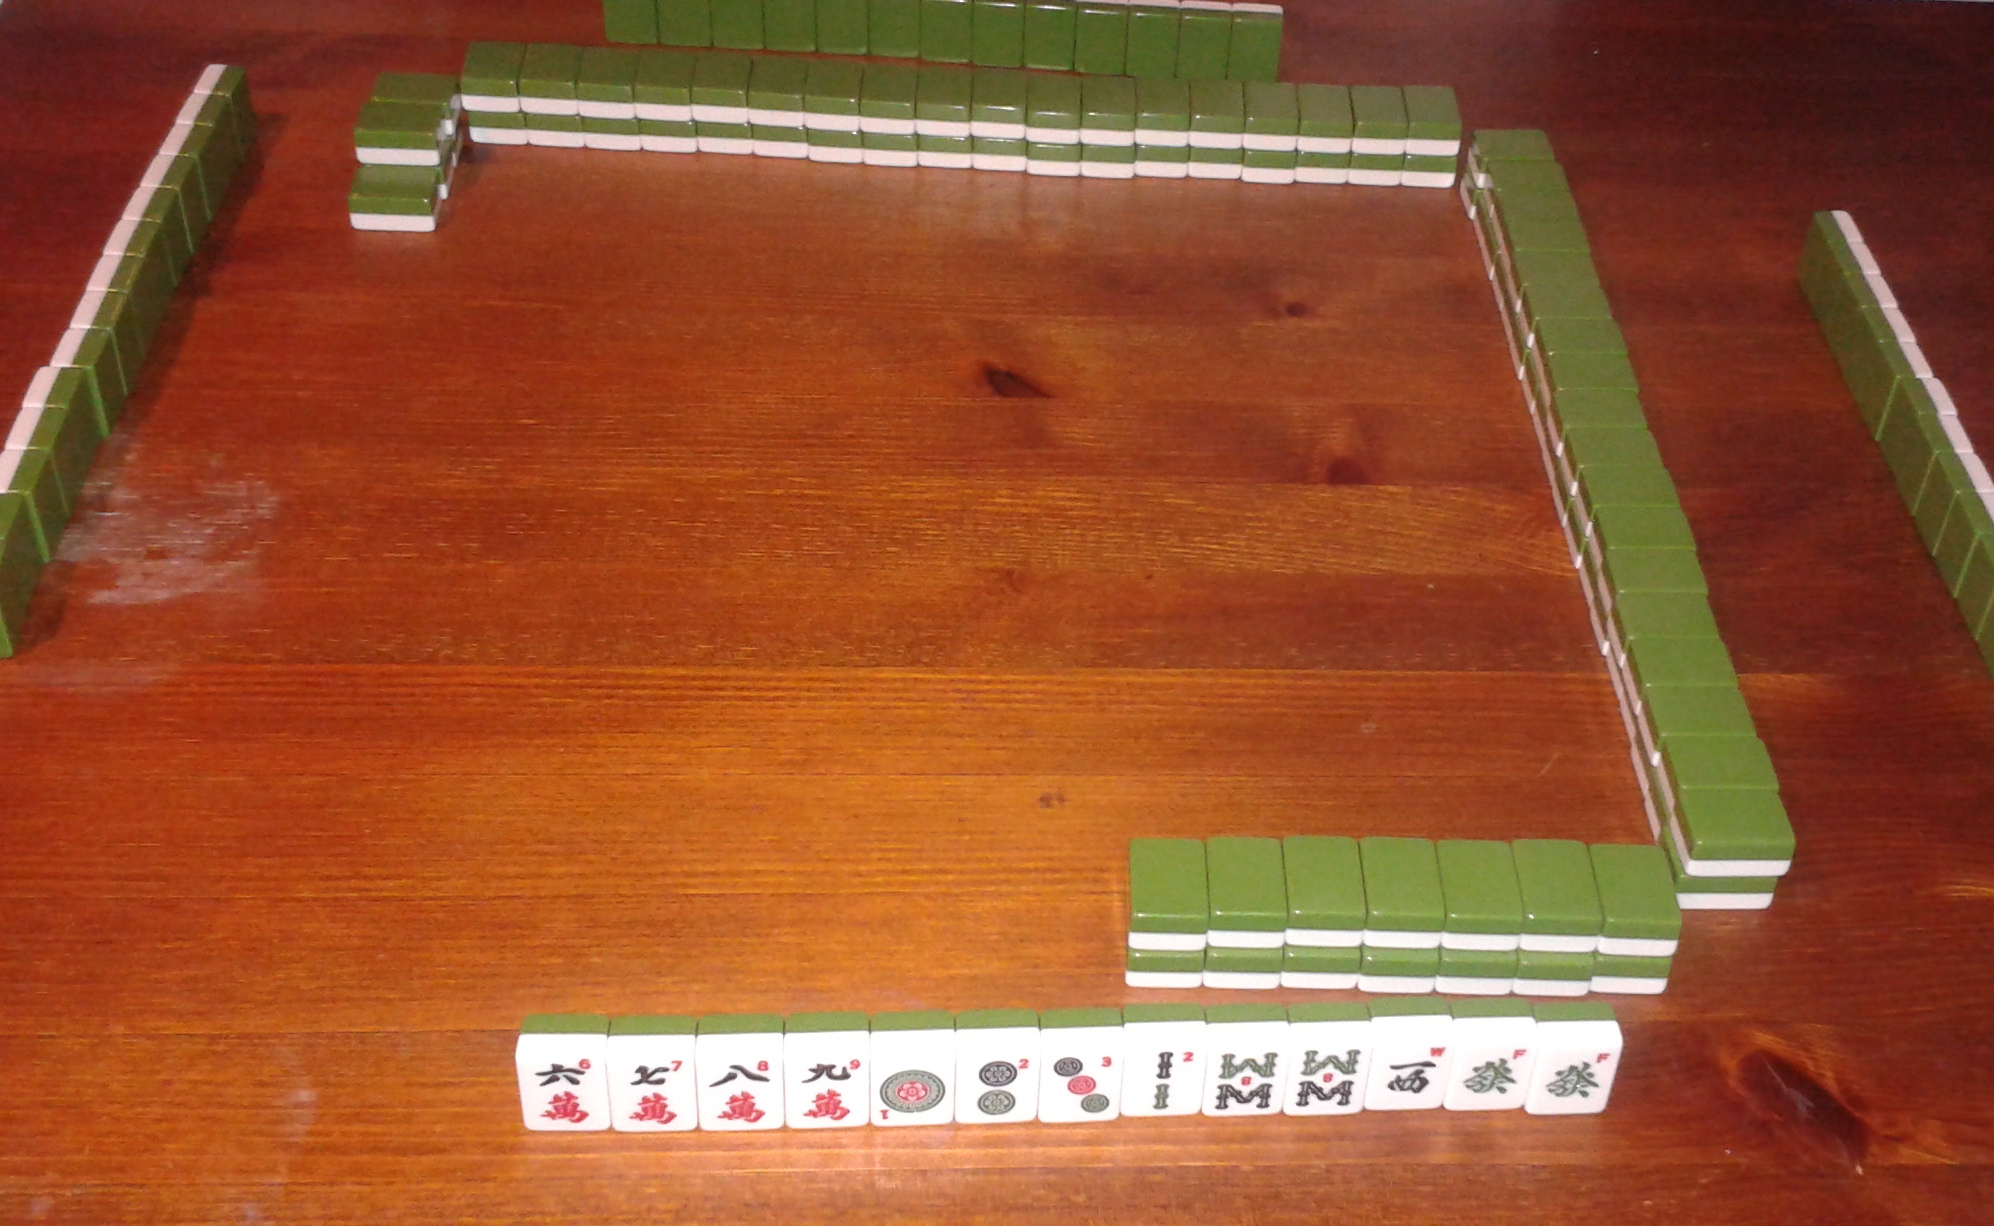
\includegraphics[width=0.75\textwidth]{mur.jpg}
\caption{Przykład sytuacji po zbudowaniu muru i rozdzieleniu kamieni pomiędzy
graczy; źródło: fotografia własna}
\label{fig:mur}
\end{figure}

\subsection{Aranżacja kamieni i deklaracje kwiatów}
Zawodnicy mogą w dowolny sposób przearanżować kamienie w swojej ręce, nie
pokazując ich pozostałym uczestnikom gry. Gracze, którzy w pierwszym przydziale
otrzymali dowolną ilość kamieni kwiatów, mogą zadeklarować \pinyin{hua} (patrz:
deklaracje na stronie \pageref{deklaracje}). Deklaracje
wykonuje się zaczynając od dilera w kierunku przeciwnym do wskazówek zegara.  
 
\subsection{Przebieg tury}
Po rozdzieleniu kamieni i deklaracji kwiatów,  gracze po kolei wykonują ruchy w
swoich turach. Pierwsza tura przysługuje dilerowi, następnie wykonują je gracze
w ruchu przeciwnym do wskazówek zegara aż do zakończenia rozdania (czyli po
kolei w cyklu gracze z przypisanym wiatrem miejsca wschodnim, południowym,
zachodnim, północnym, a następnie ponownie wschodnim).

Każdy z graczy na początku swojej tury dobiera kamień z początku muru (nie
licząc pierwszej tury dilera, który zaczyna z 1 kamieniem więcej), może dokonać
deklaracji kwiatu (jeśli takowy dobrał) lub zakrytego \pinyin{ganga} (patrz:
deklaracje na stronie \pageref{deklaracje}), a następnie deklaruje \pinyin{hu}
lub odrzuca kamień ze swojej ręki (może to być kamień właśnie przez niego dobrany). Tura
nie powinna trwać więcej niż 10 sekund.

Kamienie odrzucone należy ustawiać w rzędach o długości 6 kamieni, od lewej do
prawej, na podłodze pomiędzy ścianami muru. 

Kolejny gracz nie może rozpocząć swojej tury (dobrać kamienia z początku muru)
dopóki jego poprzednik nie odrzucił kamienia. 

Deklaracje wzięcia kamienia odrzuconego (patrz: deklaracje na stronie
\pageref{deklaracje}) powinny nastepować w odstępie kilku sekund od jego
odrzucenia, jeszcze zanim kolejny gracz zdąży rozpocząć swoją turę.

Kolejność tur zostaje zmieniona, a aktualny obieg przerwany i rozpoczęty nowy,
gdy odrzucony kamień zostanie przejęty przez innego gracza przez odpowiednią deklarację.
Wówczas rozpoczyna się tura deklarującego (przy czym zabrany przez niego kamień
zastępuje dobranie kamienia z muru), po nim tura gracza po jego prawej stronie i
tak dalej.

\subsection{Odkryte kamienie}
Po wykonaniu deklaracji \pinyin{peng}, \pinyin{gang} (wariantu odkrytego) lub
\pinyin{chi}, ręka gracza przestaje być zakryta, a przed nią
umieszczone zostają  odpowiednio trójka, \pinyin{gang} lub sekwens. W każdym z
tych 3 przypadków są to kamienie odkryte, a jeden z nich został wcześniej
odrzucony przez jednego z pozostałych graczy. W takim wypadku należy zaznaczyć,
który kamień został zabrany i który z graczy go odrzucił. Dokonuje się tego
poprzez obrócenie owego kamienia o 90 stopni i umieszczenie go:
\begin{itemize}
  \item po stronie prawej, jeśli został on zabrany od gracza po prawej stronie
  deklarującego (Rysunek \ref{fig:meldright});
  \begin{figure}[H]
  \centering
  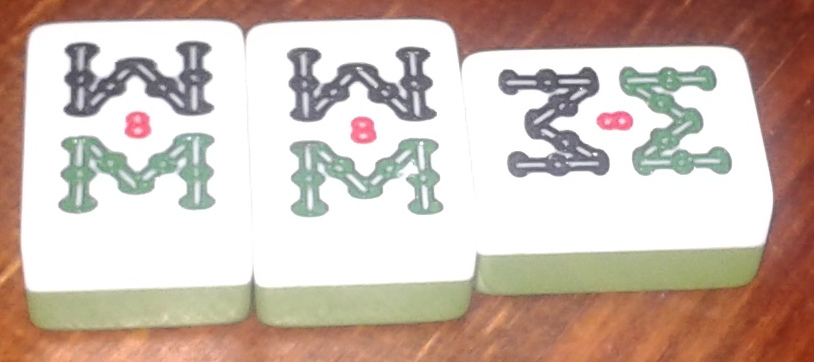
\includegraphics[width=0.50\textwidth]{meld_right.jpg}
  \caption{Przykład zgłoszenia \pinyin{peng} dla trójki złożonej z kamieni o
  numerze 8 z talii bambusów, przypadek dla kamienia zabranego od gracza po
  prawej stronie; źródło:
  fotografia własna}
  \label{fig:meldright}
  \end{figure}
  \item po stronie lewej, jeśli został on zabrany od gracza po lewej stronie
  deklarującego (Rysunek \ref{fig:meldleft});
  \begin{figure}[H]
  \centering
  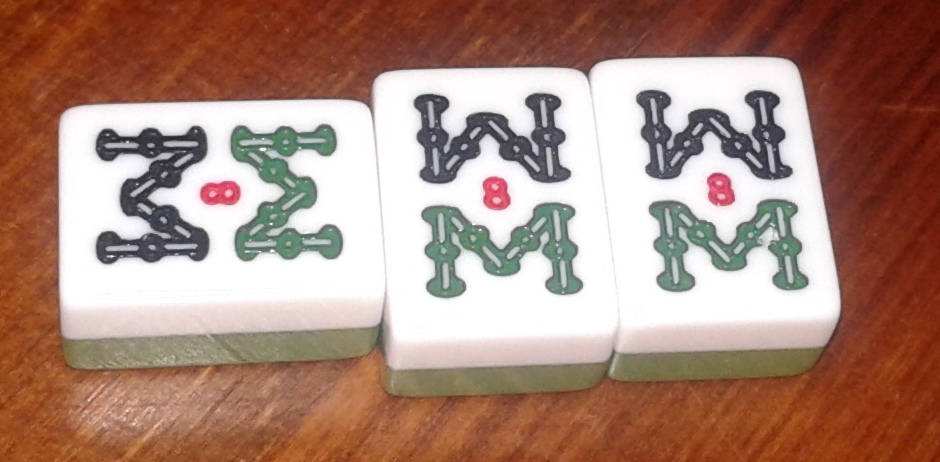
\includegraphics[width=0.45\textwidth]{meld_left.jpg}
  \caption{Przykład zgłoszenia \pinyin{peng} dla trójki złożonej z kamieni o
  numerze 8 z talii bambusów, przypadek dla kamienia zabranego od gracza po
  lewej stronie; źródło: fotografia własna}
  \label{fig:meldleft}
  \end{figure}
  \item pośrodku, jeśli został on zabrany od gracza naprzeciwko deklarującego
  (Rysunek \ref{fig:meldmid}).
  \begin{figure}[H]
  \centering
  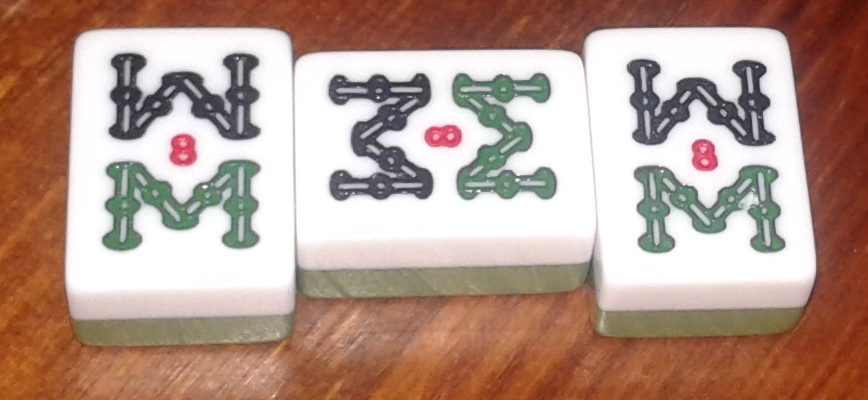
\includegraphics[width=0.45\textwidth]{meld_mid.jpg}
  \caption{Przykład zgłoszenia \pinyin{peng} dla trójki złożonej z kamieni o
  numerze 8 z talii bambusów, przypadek dla kamienia zabranego od gracza
  naprzeciwko; źródło: fotografia własna}
  \label{fig:meldmid}
  \end{figure}
\end{itemize}
% Przykłady znajdują się na Rysunku \ref{fig:meldunki} na stronie
% \pageref{fig:meldunki}.

% \begin{figure}[here]
% \centering
% 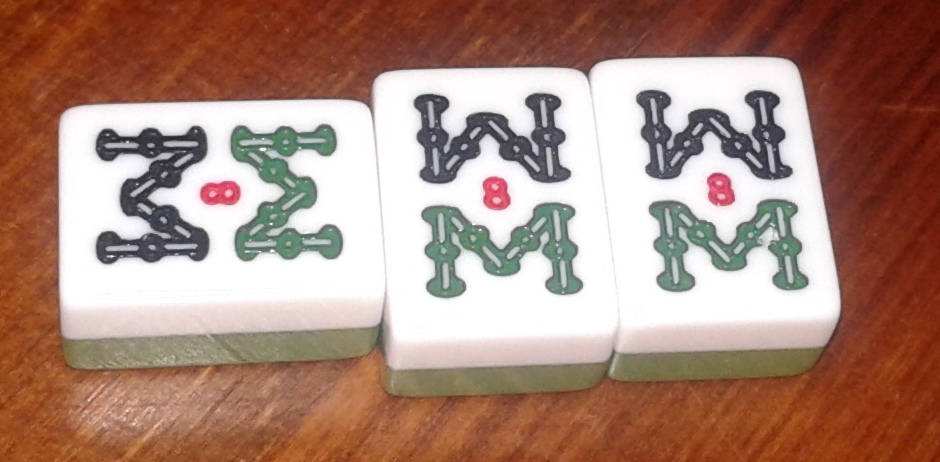
\includegraphics[width=0.75\textwidth]{meld_left.jpg}
% 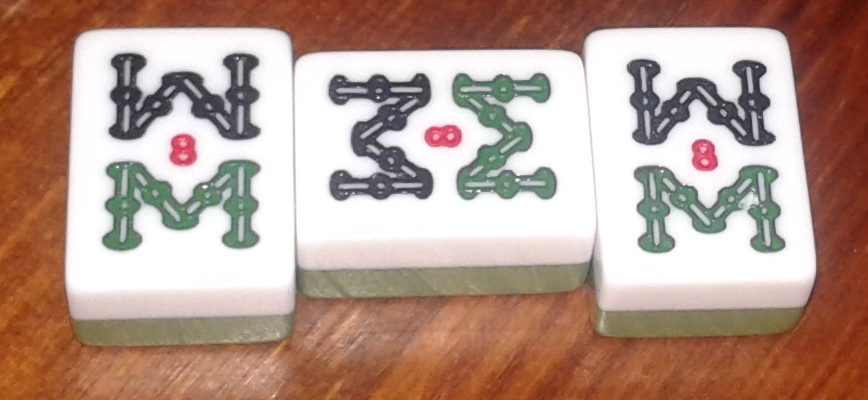
\includegraphics[width=0.75\textwidth]{meld_mid.jpg}
% 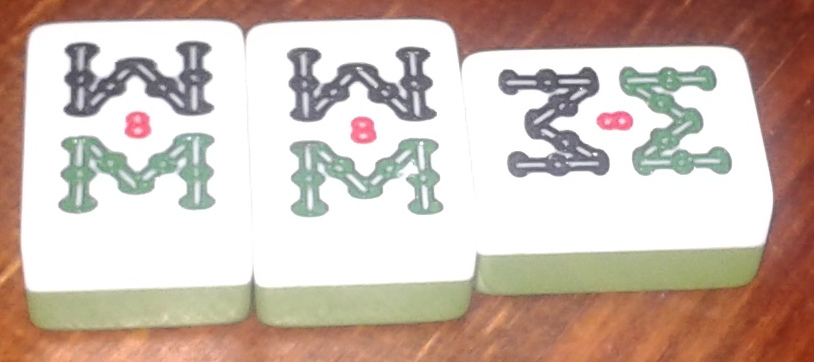
\includegraphics[width=0.75\textwidth]{meld_right.jpg}
% \caption{Przykłady zgłoszeń \pinyin{peng} dla trójki złożonej z kamieni o
% numerze 8 z talii bambusów (odpowiednio dla kamienia dobranego od gracza po
% lewej, naprzeciwko i po prawej stronie gracza); źródło: fotografie własne}
% \label{fig:meldunki}
% \end{figure}

\subsection{Zakończenie rozdania}
Rozdanie kończy się, gdy jeden z graczy zadeklaruje \pinyin{hu} lub zużyte
zostaną wszystkie kamienie w murze (dojdzie do remisu). W przypadku wygranej
zmieniają się punktacje graczy zgodnie z zasadami opisanymi na stronie
\pageref{punktacja}, natomiast przy remisie żaden z graczy nie zyskuje ani nie
traci żadnych punktów. 

Po każdym rozdaniu następuje zmiana dilera, przy czym co 4 rozdania, gdy każdy z
graczy zdążył być dilerem dokładnie raz (na początku każdej nowej rundy),
zachodzi rotacja miejsc (gracze przesiadają się na startowe miejsca przypisane
dla każdej rundy).

Jeśli zakończone rozdanie nie jest ostatnim (czwartym) rozdaniem w rundzie,
nowym dilerem w kolejnym rozdaniu staje się gracz południowy (siedzący po
prawej stronie poprzedniego dilera). Analogicznie, gracz zachodni staje się
południowym, północny -- zachodnim, a wschodni -- północnym.

Jeśli zakończone rozdanie jest ostatnim rozdaniem w rundzie, kończy się
poprzednia runda i zaczyna kolejna (nie licząc sytuacji po zakończeniu rundy
północnej, która jest ostatnią). Na początku nowej rundy następuje zmiana wiatru
rundy. Pierwsza runda to runda wschodnia, a po niej następują kolejno
południowa, zachodnia i północna. Po zakończeniu rundy północnej gra się kończy.

Przy rozpoczęciu nowej rundy następuje rotacja miejsc -- gracze wstają i
przesiadają się zgodnie z układem początkowym przypisanym dla nowej rundy.
Układy te zostały zaprojektowane w taki sposób, aby w przeciągu rozgrywki każdy
z graczy miał tyle samo okazji do deklaracji \pinyin{chi} od każdego z
pozostałych (jako że \pinyin{chi} można deklarować tylko i wyłącznie od gracza
siedzącego po lewej stronie deklarującego). Początkowe układy dla każdej z rund
to:
\begin{itemize}
  \item w rundzie wschodniej (pierwszej) gracze zaczynają na swoich początkowych
  miejscach, czyli gracz A na miejscu wschodnim, gracz B na miejscu
  południowym, gracz C na miejscu zachodnim i gracz D na miejscu północnym;
  \item w rundzie południowej (drugiej) gracz A siada na miejscu południowym,
  gracz B na miejscu wschodnim, gracz C na miejscu północnym i gracz D na
  miejscu zachodnim; 
  \item w rundzie zachodniej (trzeciej) gracz A na miejscu zachodnim, gracz B na
  miejscu północnym, gracz C na miejscu południowym i gracz D na miejscu
  wschodnim; 
  \item w rundzie północnej (czwartej) gracz A na miejscu północnym, gracz B na
  miejscu zachodnim, gracz C na miejscu wschodnim i gracz D na miejscu
  południowym.
\end{itemize}

% gówno prawda, tak jest w riichi, a nie tu
% Jeśli w rozdaniu zwyciężył diler, nie dochodzi do rotacji miejsc i rozgrywane
% jest rozdanie dodatkowe.
% 
% Jeśli w rozdaniu zwyciężył jeden z graczy pobocznych (południe, zachód lub
% północ), następuje rotacja miejsc.
% znowu: riichi 
% Gracz wschodni staje się graczem południowym,
% południowy -- zachodnim, zachodni -- północnym, a północny -- wschodnim.

% Jeśli w wyniku rotacji miejsc nowy gracz wschodni byłby nim po raz drugi w tej
% rundzie (nie licząc rozdań dodatkowych), rozpoczyna się nowa runda (lub, w
% przypadku rundy północnej, zakończona zostaje kompletna gra) i zmienia się
% wiatr rundy. Zmiana wiatru rundy następuje analogicznie do rotacji miejsc, czyli
% po rundzie wschodniej następuje południowa, po południowej -- zachodnia, a po
% zachodniej -- północna. Runda północna jest ostatnią.

\section{Deklaracje}
\label{deklaracje}
W czasie gry przy wszystkich akcjach pozwalających dobrać kamień odrzucony przez
innego gracza (\peng, \dekchi, \hu lub \gang) lub kamień uzupełniający z końca
muru (\pinyin{gang} lub \hua) jest absolutnie obowiązkowym, aby głośno
wypowiedzieć ich deklaracje. Przykładowo, gdy gracz chce dobrać kamień odrzucony przez innego
gracza do własnej trójki, musi głośno powiedzieć ,,\peng'', natomiast gdy chce
go użyć do sekwensu, nie może tego uczynić nie mówiąc ,,\dekchi''. 

Jednakże, gracze nie powinni deklarować nazw kamieni przez nich odrzucanych, a
dyskusja na temat przebiegu gry w jej trakcie jest całkowicie zakazana.

Deklaracje występujące w grze: 
\begin{itemize}
  \item \deklaracja{peng}
  gdy gracz posiada parę danego kamienia (2 jego wystąpienia), a jeden z
  pozostałych uczestników gry odrzuci jego trzeci egzemplarz, posiadacz pary
  może zadeklarować głośno ,,\pinyin{peng}'', zabrać odrzucony kamień, odkryć
  swoją parę i traktować te 3 kamienie jako własną trójkę; deklaracja
  \pinyin{peng} przerywa obieg, zmienia kolejność tur i czyni deklarującego
  aktywnym graczem (musi on w następnej kolejności odrzucić kamień; nie dobiera
  on z muru, jako że otrzymał już kamień wykonując \pinyin{peng});
  \item \deklaracja{gang}
  istnieją 2 sposoby deklaracji \pinyin{gang}:
    \begin{itemize}
    \item odkryty \deklaracja{gang}
    gdy gracz posiada trójkę danego kamienia (3 jego wystąpienia), a jeden z
    pozostałych uczestników gry odrzuci jego czwarty (i tym samym, ostatni)
    egzemplarz, posiadacz trójki może zadeklarować głośno ,,\pinyin{gang}'',
    zabrać odrzucony kamień, odkryć swoją trójkę i traktować te 4 kamienie jako
    własnego \pinyin{ganga} (czwórkę); ten sposób deklaracji \pinyin{gang}
    przerywa obieg, zmienia kolejność tur i czyni deklarującego aktywnym graczem;
    \item zakryty \deklaracja{gang} \label{closed_gang}
    gdy gracz posiada zakryte 4 wystąpienia danego kamienia, może zadeklarować
    głośno ,,\pinyin{gang}'', położyć je zakryte poziomo przed swoją ręką i
    traktować jako \pinyin{ganga} (czwórkę); ten sposób deklaracji zapobiega
    odkryciu ręki;
    \item niezależnie od sposobu deklaracji \pinyin{gang}, po jej wykonaniu
    gracz powinien dobrać kamień uzupełniający z końca muru (w przypadku
    deklaracji odkrytego \pinyin{ganga}, powinien to zrobić przed odrzuceniem
    kamienia);
    \end{itemize}
  \item \deklaracja{chi}
  gdy gracz posiada 2 z 3 kamieni tworzących sekwens, a jeden z pozostałych
  uczestników gry odrzuci 3ci, dopełniający go, można zadeklarować
  głośno ,,\pinyin{chi}'', zabrać odrzucony kamień, odkryć cały sekwens i
  traktować go jako własny; deklaracja
  \pinyin{chi} przerywa obieg, zmienia kolejność tur i czyni deklarującego
  aktywnym graczem (musi on w następnej kolejności odrzucić kamień; nie dobiera
  on z muru, jako że otrzymał już kamień wykonując \pinyin{chi});
  \item \deklaracja{hu}
  gdy gracz ułoży rękę spełniającą kryteria wygranej (patrz: strona
  \pageref{wygrywajacareka}), może głośno zadeklarować ,,\pinyin{hu}'', kończąc
  tym samym rozdanie, odkryć swoje kamienie, a następnie podliczyć należne mu punkty
  (patrz: strona \pageref{punktacja}); można to zrobić, gdy wygrana ręka
  zostanie skompletowana poprzez dobranie wygrywającego kamienia z muru
  (\pinyin{zimo}) lub gdy zostanie on odrzucony przez jednego z pozostałych
  graczy (zabierając go, analogicznie jak przy deklaracji \pinyin{peng} lub
  \pinyin{gang}); w przypadku, gdy 2 lub 3 graczy zadeklaruje \pinyin{hu} na
  jednym kamieniu (odrzuconym przez innego gracza), zwycięża tylko jeden z nich,
  zajmujący miejsce najbliższe w kolejce tur względem gracza odrzucającego
  kamień, na którym padły deklaracje;
  \item \deklaracja{hua}
  gdy gracz dobierze z muru kamień kwiatu (lub zacznie z takowym na ręce
  początkowej w rozdaniu), może zadeklarować głośno ,,\pinyin{hua}'', odkryć
  go, umieścić przed swoją zakrytą ręką, a następnie dobrać kamień uzupełniający
  z końca muru; każdy kamień kwiat zadeklarowany w ten sposób zwiększa końcową
  wartość ręki o 1 punkt.
\end{itemize}

\section{\pinyin{Fan}}
\label{fan}
Istnieje 81 układów punktowanych \pinyin{fan}, z których każdy z nich ma
przypisaną jedną z 12 wartości punktowych: 88, 64, 48, 32, 24, 16, 12, 8, 6, 4,
2 lub 1. Dana ręka
wygrywająca może spełniać więcej niż jedno \pinyin{fan} i aby gracz mógł w
poprawny sposób zadeklarować z nią \pinyin{hu}, muszą one być łącznie warte co
najmniej 8 punktów (z wyłączeniem punktów za kamienie kwiatów).

Istnieje 5 zasad dotyczących interpretacji \pinyin{fan}:
\begin{itemize}
  \item brak powtórzeń -- jeśli jedno \pinyin{fan} jest implikowane przez
  drugie, nie można policzyć punktów za oba\footnote{Dla przykładu,
  \pinyin{fan} Trzy Małe Smoki implikuje Trójkę ze Smoków, w związku z
  czym gracz może użyć tylko jednego z tych dwóch \pinyin{fan} przy podliczaniu
  punktów.};
  \item brak separacji -- jeśli kamienie na ręce zostały podzielone na grupy
  (trójki, sekwensy lub \pinyin{gangi}) w jeden sposób na potrzeby spełnienia
  jednego \pinyin{fan}, nie mogą w następnej kolejności zostać podzielone w inny
  sposób, na potrzeby innego \pinyin{fan};
  \item rozróżnienie -- jeśli dana grupa (trójka, sekwens lub \pinyin{gang})
  została użyta na potrzeby uzyskania konkretnego \pinyin{fan}, nie może ona
  zostać użyta ponownie wraz z innymi grupami do uzyskania tego samego
  \pinyin{fan};
  \item wybór dowolnego wyniku -- jeśli daną rękę można zinterpretować różnymi
  zestawami \pinyin{fan}, w wyniku czego może ona być warta różne liczby
  punktów, gracz ma prawo zdecydować się na wyżej punktowaną z opcji;
  \item wyłączność -- jeśli pewne grupy (trójki, sekwensy lub \pinyin{gangi})
  zostały użyte do uzyskania jednego \pinyin{fan}, pozostałe kamienie mogą
  zostać połączone z jedną z owych grup do uzyskania innego \pinyin{fan} tylko 1
  raz.
\end{itemize}

Tablica wszystkich układów (tablica \ref{tab:fan}) znajduje się w suplemencie na stronie \pageref{tab:fan2}.

\section{Punktacja}
\label{punktacja}
Na punktację wygrywającej ręki po deklaracji \pinyin{hu} jej właściciela
składają się 3 rodzaje punktów: 
\begin{itemize}
  \item punkty podstawowe -- suma wszystkich fan, które spełnia ręka (zgodnie z
  zasadami opisanymi w sekcji \ref{fan} na stronie \pageref{fan});
  \item punkty dodatkowe -- 8 punktów, które każdy z graczy, którzy nie wygrali,
  musi zapłacić zwycięzcy (niezależne od \pinyin{fan});
  \item punkty karne -- jeśli w trakcie rozdania zwycięzca złamał jedną z zasad,
  przydzielane są mu odpowiednie punkty ujemne (mogą one zostać przydzielone na
  końcu gry lub po rozliczeniu całego rozdania - patrz: sekcja
  \ref{penalties} na stronie \pageref{penalties}).
\end{itemize}

Wartość ręki można opisać następującymi wzorami:

(S -- łączna wartość ręki, d -- punkty dodatkowe, p -- punkty podstawowe)
\begin{itemize}
  \item w przypadku wygranej \pinyin{zimo} (kamień wygrywający dobrany z muru):
  	\begin{equation*}
		S = 3(d + p)
		\label{zimo}
	\end{equation*}
	każdy z pozostałych graczy płaci zwycięzcy punkty dodatkowe oraz podstawowe;
  \item w przypadku wygranej \pinyin{dian} (kamień wygrywający dobrany od
  innego gracza):
  	\begin{equation*}
		S = 3d +p
		\label{dian}
	\end{equation*}
	każdy z pozostałych graczy płaci zwycięzcy punkty dodatkowe, ale tylko gracz,
	którego odrzucony kamień był kamieniem wygrywającym, płaci punkty podstawowe.
\end{itemize}

\section{Kary}
\label{penalties}
Zachowania niezgodne z zasadami gry, niezależnie czy świadome, czy przypadkowe,
mogą zakończyć się ostrzeżeniem, ale też utratą puktów, prawa do zwycięstwa w
aktualnie rozgrywanym rozdaniu (tzw. ,,martwą ręką'' - ręką, która nie może
zostać ukończona), a nawet (w przypadku cięższych przewinień na zawodach
sportowych) utratą praw do udziału w przyszłych turniejach, anulowaniem
kwalifikacji i miejsc w rankingach oraz otwartą krytyką.

Arbiter ma prawo ukarać gracza za łamanie zasad, orzekając 5, 10, 20, 30, 40,
50 lub 60 punktów karnych, zgodnie z własnym osądem na podstawie powagi
przewinienia. Owe punkty zostają odjęte od puli ukaranego gracza, lecz nie są
dodawane do punktów pozostałych graczy przy tym samym stole (jak w przypadku
innych rodzajów punktów).

Konkretne przypadki złamanych zasad wraz z adekwatną do nich karą:
\begin{itemize}
  \item oszustwo -- arbiter ma prawdo do dyskwalifikacji gracza z zawodów, jeśli
  podmieniał on którekolwiek z kamieni biorące udział w grze w dowolny sposób
  nie będący częścią procesu gry;
  \item gracz, który niepoprawnie zgłosił \pinyin{chi}, \pinyin{peng},
  \pinyin{gang} lub \pinyin{hua}, jest karany martwą ręką;
  \item puste deklaracje -- deklaracja \pinyin{chi}, \pinyin{peng}
  lub \pinyin{gang}, po której gracz następnie ją cofa i rezygnuje z wykonania
  adekwatnej akcji, nazywana jest ,,pustą deklaracją''; pierwszy przypadek
  takiej deklaracji karany jest ostrzeżeniem, drugi -- 5 punktami karnymi, a
  każdy kolejny dwukrotnością poprzedniej kary (czyli trzeci -- 10 punktów
  karnych, czwarty -- 20 i tak dalej);
  \item dotknięcie kamienia z muru zanim gracz poprzedzający odrzucił swój
  kamień karane jest ostrzeżeniem przy pierwszym wystąpieniu, 5 punktami karnymi
  przy drugim, a każdy kolejny przypadek dwukrotnością poprzedniej kary (czyli
  trzeci -- 10 punktów karnych, czwarty -- 20 i tak dalej); jeśli dotknięty w
  taki sposób kamień zostaje w efekcie odkryty, gracz ukarany jest także martwą ręką;
  \item deklaracja \pinyin{peng} później niż 3 sekundy po odrzuceniu kamienia
  karana jest ostrzeżeniem przy pierwszym wystąpieniu, 5 punktami karnymi
  przy drugim, a każdy kolejny przypadek dwukrotnością poprzedniej kary (czyli
  trzeci -- 10 punktów karnych, czwarty -- 20 i tak dalej);
  \item fałszywe \pinyin{hu} karane jest zależnie od okoliczności:
  	\begin{itemize}
  	  \item gdy wartość ręki jest mniejsza od 8 punktów lub kamień, który został
  	  uznany przez gracza za jego kamień wygrywający, tak naprawdę nim nie był,
  	  gracz przekazuje po 10 punktów do puli każdego z pozostałych graczy przy
  	  stole oraz jest ukarany martwą ręką;
  	  \item gdy gracz deklaruje \pinyin{hu}, jednakże jego ręka nie znajdowała
  	  się w stanie czekania (brakowało mu więcej niż jednego kamienia do
  	  wygranej), przekazuje on po 20 punktów do puli każdego z pozostałych graczy
  	  przy stole oraz jest ukarany martwą ręką;
  	\end{itemize}
  \item w przypadku, gdy gracz omyłkowo odsłoni jeden ze swoich kamieni, jest on
  zmuszony odrzucić go w czasie swojej następnej tury jako karny kamień;
  \item w przypadku, gdy gracz omyłkowo odsłoni jeden z kamieni pozostałych
  graczy, otrzymuje on punkty karne w wysokości od 5 do 60 punktów, zależnie od
  decyzji arbitra;
  \item jeśli gracz odsłoni wszystkie swoje kamienie po prawidłowej deklaracji
  \pinyin{hu} innego uczestnika gry, karany jest ostrzeżeniem; jednakże, jeśli
  było to falszywe \pinyin{hu}, zamiast ostrzeżenia, karą jest martwa ręka i
  konieczność odrzucenia wszystkich odsłoniętych wówczas kamieni w dowolnej
  kolejności, jeden za drugim, aż wszystkie zostaną odrzucone i zastąpione
  nowymi kamieniami dobranymi z muru; ponadto, jeśli przy okazji odsłonięcia
  swojej ręki w podobnej sytuacji odsłonięte zostały również kamienie z muru lub
  kamienie innych graczy i w rezultacie dalsze rozgrywanie aktualnego rozdania
  nie jest możliwe, gracz zmuszony jest przekazać po 30 punktów do puli każdego
  z pozostałych graczy przy stole (na podstawie decyzji arbitra);
  \item gracz posiadający nieprawidłową liczbę kamieni na ręce karany jest
  martwą ręką w danym rozdaniu;
  \item przekazywanie informacji o przebiegu gry (fałszywych lub prawdziwych --
  na przykład dotyczących konkretnych kamieni zawartych na własnej ręce)
  skutkuje martwą ręką w danym rozdaniu;
  \item utrudnianie gry i pracy arbitra może skutkować dyskwalifikacją z gry.
\end{itemize}



\chapter{Zestawienie najważniejszych wariantów zasad gry}
\label{zestawienie_zasad}
\section{Różnorodność zasad gry w madżonga w Chinach i na świecie}
\epigraph{麻将源于中国属于世界 \\ 
\footnotesize \pinyin{Májiàng yuán yú Zhōngguó shǔyú shìjiè} \normalsize \\
Mahjong pochodzi z Chin, lecz
należy do świata.}{Yu Guangyuan\footnote{Yu Guangyuan (于光远 Yú
Guāngyuǎn) (1915-2013) -- znany chiński filozof i działacz Komunistycznej Partii
Chin; prezes Światowej Organizacji Madżonga w latach 2005 do 2013 (Sina
Xīnlàng Lùntán 2010; Wikipedia 2016).}
\\ (Shìjiè Májiàng Zǔzhī 2014)}

Aktualnie na świecie istnieje kilkadziesiąt rozróżnialnych zestawów zasad gry
w madżonga. W wielu przypadkach gracze pochodzący z danego obszaru nie są
nawet świadomi istnienia innych wariantów niż ten, w który grają sami. Według
klasyfikacji Toma Slopera jest ich 42 (Sloper 2002), jednakże nie uwzględnia on
wielu spośród mniej znanych lub różniących się od nich drobnymi szczegółami, jak
choćby odmiana południowoafrykańska (zbliżona do zasad, zgodnie z którymi gra
się w Hongkongu) (World Series of Mahjong 2015).

Warto także wspomnieć, że nawet współcześnie powstają nowe warianty gry, które
cieszą się zainteresowaniem wprowadzając innowacyjne zasady, jednakże przestrzegając w
wystarczającym stopniu tych istniejących wcześniej, aby wciąż klasyfikowano je
jako reguły gry w madżonga. \label{washizu} Przykładem takich zasad jest
japoński madżong \romaji{washizu} (鷲巣), zwany również madżongiem transparentnym
(麻雀透明 \romaji{mājan tōmei}). Pochodzi on z mangi pod tytułem \textit{,,Akagi:
Geniusz, który zstąpił w ciemność''} (アカギ闇に降り立った天才 \romaji{Akagi:} \romaji{Yami}
\romaji{ni} \romaji{Oritatta} \romaji{Tensai}), która jest wciąż wydawana od
1992 roku przez \mbox{Nobuyuki} \mbox{Fukumoto} (福本伸行 \mbox{Fukumoto}
\mbox{Nobuyuki}).
Esencją sukcesu \romaji{washizu} jest zmiana trzech czwartych kamieni na transparentne, co
drastycznie zmienia przebieg rozgrywki. Pomijając tę zmianę i sposób podziału
kamieni, madżong transparentny w zasadzie nie różni się od japońskich zasad
turniejowych \romaji{rīchi},
% (patrz:strona \pageref{rīchi})
jednakże mimo to stał się on popularny na całym świecie. Podobnych przykładów
powstających współcześnie i zyskujących rozgłos nowych zasad gry w madżonga jest
wiele (Miller 2015).

W związku z mnogością różnorodnych zasad autor nie opisze ich wszystkich w
treści niniejszej pracy, skupiając się na tych z nich, które współcześnie są
najpopularniejsze lub miały historycznie największy wpływ na kulturę gry w
madżonga. Jako punkt odniesienia w ich zestawianiu potraktowane zostaną
międzynarodowe zasady turniejowe, których szczegółowy opis znajduje się w
rozdziale \ref{guobiao}.
%  oraz skróconym
% scharakteryzowaniu 6 innych spośród najpopularniejszych i najbardziej wpływowych
% wariantów (patrz: strona \pageref{inne_zasady}). 

\section{Madżong chiński klasyczny}
\label{cc}
\def \refpodwariantycc {\getrefnumber{podwarianty_cc}} 
%\subsection{Historia}
Na przełomie XIX i XX wieku (patrz: rozdział \ref{historia}) nastąpiło
przekształcenie licznych gier karcianych w pierwsze postaci madżonga. Ze względu
na brak spisanych i ustalonych reguł w tym okresie występowało wiele
rozbieżności w kwestii stosowanych zasad.
Pierwsze próby standaryzacji nastąpiły w latach dwudziestych
XX wieku w Szanghaju (patrz: strona \pageref{shanghai20s}). Naturalnie, pomiędzy
samymi zasadami ustandaryzowanymi przez różnych piszących w tym czasie autorów
również występowały pewne rozbieżności, jednakże wszystkie one są łącznie
określane jako ,,zasady chińskie klasyczne'' (Sloper 2006).

Nie jest pewne, czy zasady klasyczne są najstarszymi zasadami,
choć jest to bardzo prawdopodobne (więcej na ten temat w sekcji \ref{ccvshkos}
na stronie \pageref{ccvshkos}).

Wyjaśnienie najważniejszych, szczególnych cech zasad chińskich klasycznych w
dalszej części tej sekcji wykonane zostało na podstawie ich 3
najważniejszych podwariantów wyszczególnionych w ,,Amerykańskim Kodeksie Praw
Madżonga'' (Babcock \& Foster \& Hartman \& Smith \& Work 1924), nazywanych
dalej (zgodnie z nazewnictwem stosowanym w kodeksie)
\foreign{Mixed-Hand}\footnote{\label{podwarianty_cc}Nazwy 3 wymienionych
podwariantów pochodzą od wymagań narzuconych dla wygrywającej ręki w każdym z
nich. \foreign{Mixed-Hand} to dosłownie ,,mieszana ręka'' (brak restrykcji
względem używanych kamieni), \foreign{One-Double} to ,,jedno podwojenie'' (jeden
obowiązkowy mnożnik na wygrywającej ręce), natomiast \foreign{Cleared-Hand} --
,,wyczyszczona ręka'' (wymagana jest czysta ręka składająca się z tylko jednego
typu kamieni oraz opcjonalnie honorów).},
\foreign{One-Double}\footnotemark[\refpodwariantycc] oraz
\foreign{Cleared-Hand}\footnotemark[\refpodwariantycc].

Wiatr miejsca (a tym samym miejsce przy stole gracza) przydzielany jest poprzez
zmieszanie ze sobą 4 różnych kamieni wiatrów a następnie dobranie po jednym
przez każdego z graczy (osoba mieszająca kamienie bierze ostatni kamień).

\label{cc_mixed_hand}
W czasie konstrukcji muru w podwariancie \foreign{Mixed-Hand} (ale nie w
\foreign{One-Double} oraz \foreign{Cleared-Hand}) z jego części wydzielany jest
tak zwany ,,martwy mur''. Tym mianem określa się 14 kamieni od końca muru, z
których nie można dobierać w procesie gry w zwyczajnym procesie tury, lecz
jedynie jako uzupełnienia kwiatów oraz \pinyin{gangów}. Tym samym, ostatnim
dostępnym kamieniem na potrzeby konkretnych układów jest piętnasty kamień od
końca muru, a nie pierwszy, jak w przypadku międzynarodowych zasad turniejowych.

Zestaw do gry składa się ze 144  lub 136 kamieni (kamienie kwiatów są
opcjonalne -- w przypadku ich braku każdy z boków muru jest o 1 kamień krótszy,
czyli ma długość 17 kamieni). Kamienie kwiatów i pór roku są rozróżniane między
sobą -- zebranie 4 pór roku lub 4 pozostałych kwiatów przez jednego gracza
nazywane jest ,,bukietem''.

Zamiast rotacji miejsc stosowanej w przypadku międzynarodowych zasad
turniejowych, gracze przekazują wiatr miejsca w kierunku przeciwnym do wskazówek
zegara po każdym rozdaniu, w którym nie zwyciężył gracz wschodni (czyli na
początku każdej nowej rundy wiatr wschodni przypisany jest do tego samego
gracza). W przypadku gdy w rozdaniu zwycięży gracz z przypisanym wiatrem
wschodnim, wiatry miejsc nie ulegają przesunięciu i rozgrywane jest dodatkowe
rozdanie (innymi słowy, runda składa się ze zmiennej liczby rozdań -- 4 + liczba
zwycięstw wiatru wschodniego w tej rundzie).

Informacje o kolejności odrzuconych kamieni oraz o pochodzeniu kamieni dobranych
po deklaracjach od innych graczy nie są przechowywane na stole. Odrzucone
kamienie odrzucane są na podłogę pomiędzy ścianami muru w nieuporządkowany
sposób, a w przypadku sekwensów, trójek i \pinyin{gangów} nie ma potrzeby
oznaczania od kogo został dobrany brakujący kamień. 

Układy punktowane dzielą się na podstawowe (które są sumowane przy wygranej)
oraz podwajające. Każdy układ podwajający pozwala przemnożyć sumę punktów
podstawowych przez 2. Innymi słowy, stosowany jest następujący wzór (S -- łączna
wartość ręki; suma -- suma punktów podstawowych; n -- liczba układów
podwajających):
	\begin{equation*}
		S = suma \times 2^n
		\label{zimo}
	\end{equation*}

Wygrywająca ręka, podobnie jak w prawie wszystkich odmianach współczesnego
madżonga, musi składać się z 4 zestawów (trójek, sekwensów lub \pinyin{gangów})
oraz pary. W przypadku najprostszego podwariantu -- \foreign{Mixed-hand} , nie
ma żadnych dalszych restrykcji. \foreign{One-Double} wymaga, aby ręka spełniała co
najmniej jeden z układów podwajających (za wyjątkiem kamieni kwiatów), natomiast
przy \foreign{Cleared-Hand} niezbędne jest, aby ręka używała tylko jednej talii
(z albo bez honorów), samych honorów lub tylko kamieni terminalnych.

Podsumowując, zasady klasyczne zawierają w sobie dużo wyższy czynnik hazardowy,
wygrana jest zdecydowanie bardziej zależna od przypadku, niż ma to miejsce w
przypadku zasad stosowanych współcześnie na zawodach sportowych. Jednakże, wciąż
cieszą się one pewną popularnością, jako że nie są tak skomplikowane, jak wiele
powstałych później wariantów zasad, a wciąż zawierają wszystkie najważniejsze
elementy rozgrywki, przez co często są wykorzystywane jako zasady szkoleniowe.

%TODO: hong kong new style 
\section{Madżong kantoński}
\label{hkos}
Madżong kantoński, znany również jako hongkoński, występuje w 2 różnych
odmianach, zwanych ,,starym stylem'' (lub po prostu ,,starymi zasadami) oraz
,,nowym stylem''.

Nie jest niczym zaskakującym, że na terenie Kantonu (ale nie w Hong Kongu) w
czasie gry używa się kantońskiej wymowy deklaracji, nazw kamieni i układów.
Należy jednakże mieć na uwadze, że nie wszystkie wersje kantońskie są czytaniami
tych samych znaków -- dla przykładu, przy deklaracji \pinyin{chi} w Kantonie
używa się słowa \jyutping{seon} (順 \jyutping{seon6}), a nie \jyutping{hek} (喫
\jyutping{hek3}) (Rep 2006).

Jako że w Hong Kongu hazard nie jest zakazany, madżong kantoński (również w
nowym stylu) nigdy nie utracił cech gry hazardowej. %TODO: źródlo

\subsection{Stary styl}
Wiele wskazuje na to, że ten zestaw zasad jest nie tylko jednym ze starszych,
ale wręcz jest najstarszym ze wszystkich, choć wciąż jest to przedmiotem
nierozstrzygniętej dyskusji (więcej na ten temat w sekcji \ref{ccvshkos} na
stronie \pageref{ccvshkos}). Do dzisiaj jest on rozpowszechniony nie tylko w
Kantonie i Hong Kongu, lecz na całym świecie.

Sam proces gry różni się jedynie detalami od madżonga klasycznego.
Przykładowo, zakryty \pinyin{gang} po deklaracji składa się (wbrew nazwie) z
odkrytych kamieni (podczas gdy w madżongu klasycznym i większości innych
odmian, tylko 2 wewnętrzne kamienie są odkryte, natomiast zgodnie z
międzynarodowymi zasadami turniejowymi wszystkie 4 kamienie muszą być zakryte
-- patrz: Rysunek \ref{fig:closed_gang_options} oraz zasady międzynarodowe
turniejowe na stronie \pageref{closed_gang}).
Występuje więcej podobnych, drobnych różnic, lecz w większości nie mają one dużego wpływu na przebieg
rozgrywki.

\begin{figure}[H]
  \centering
  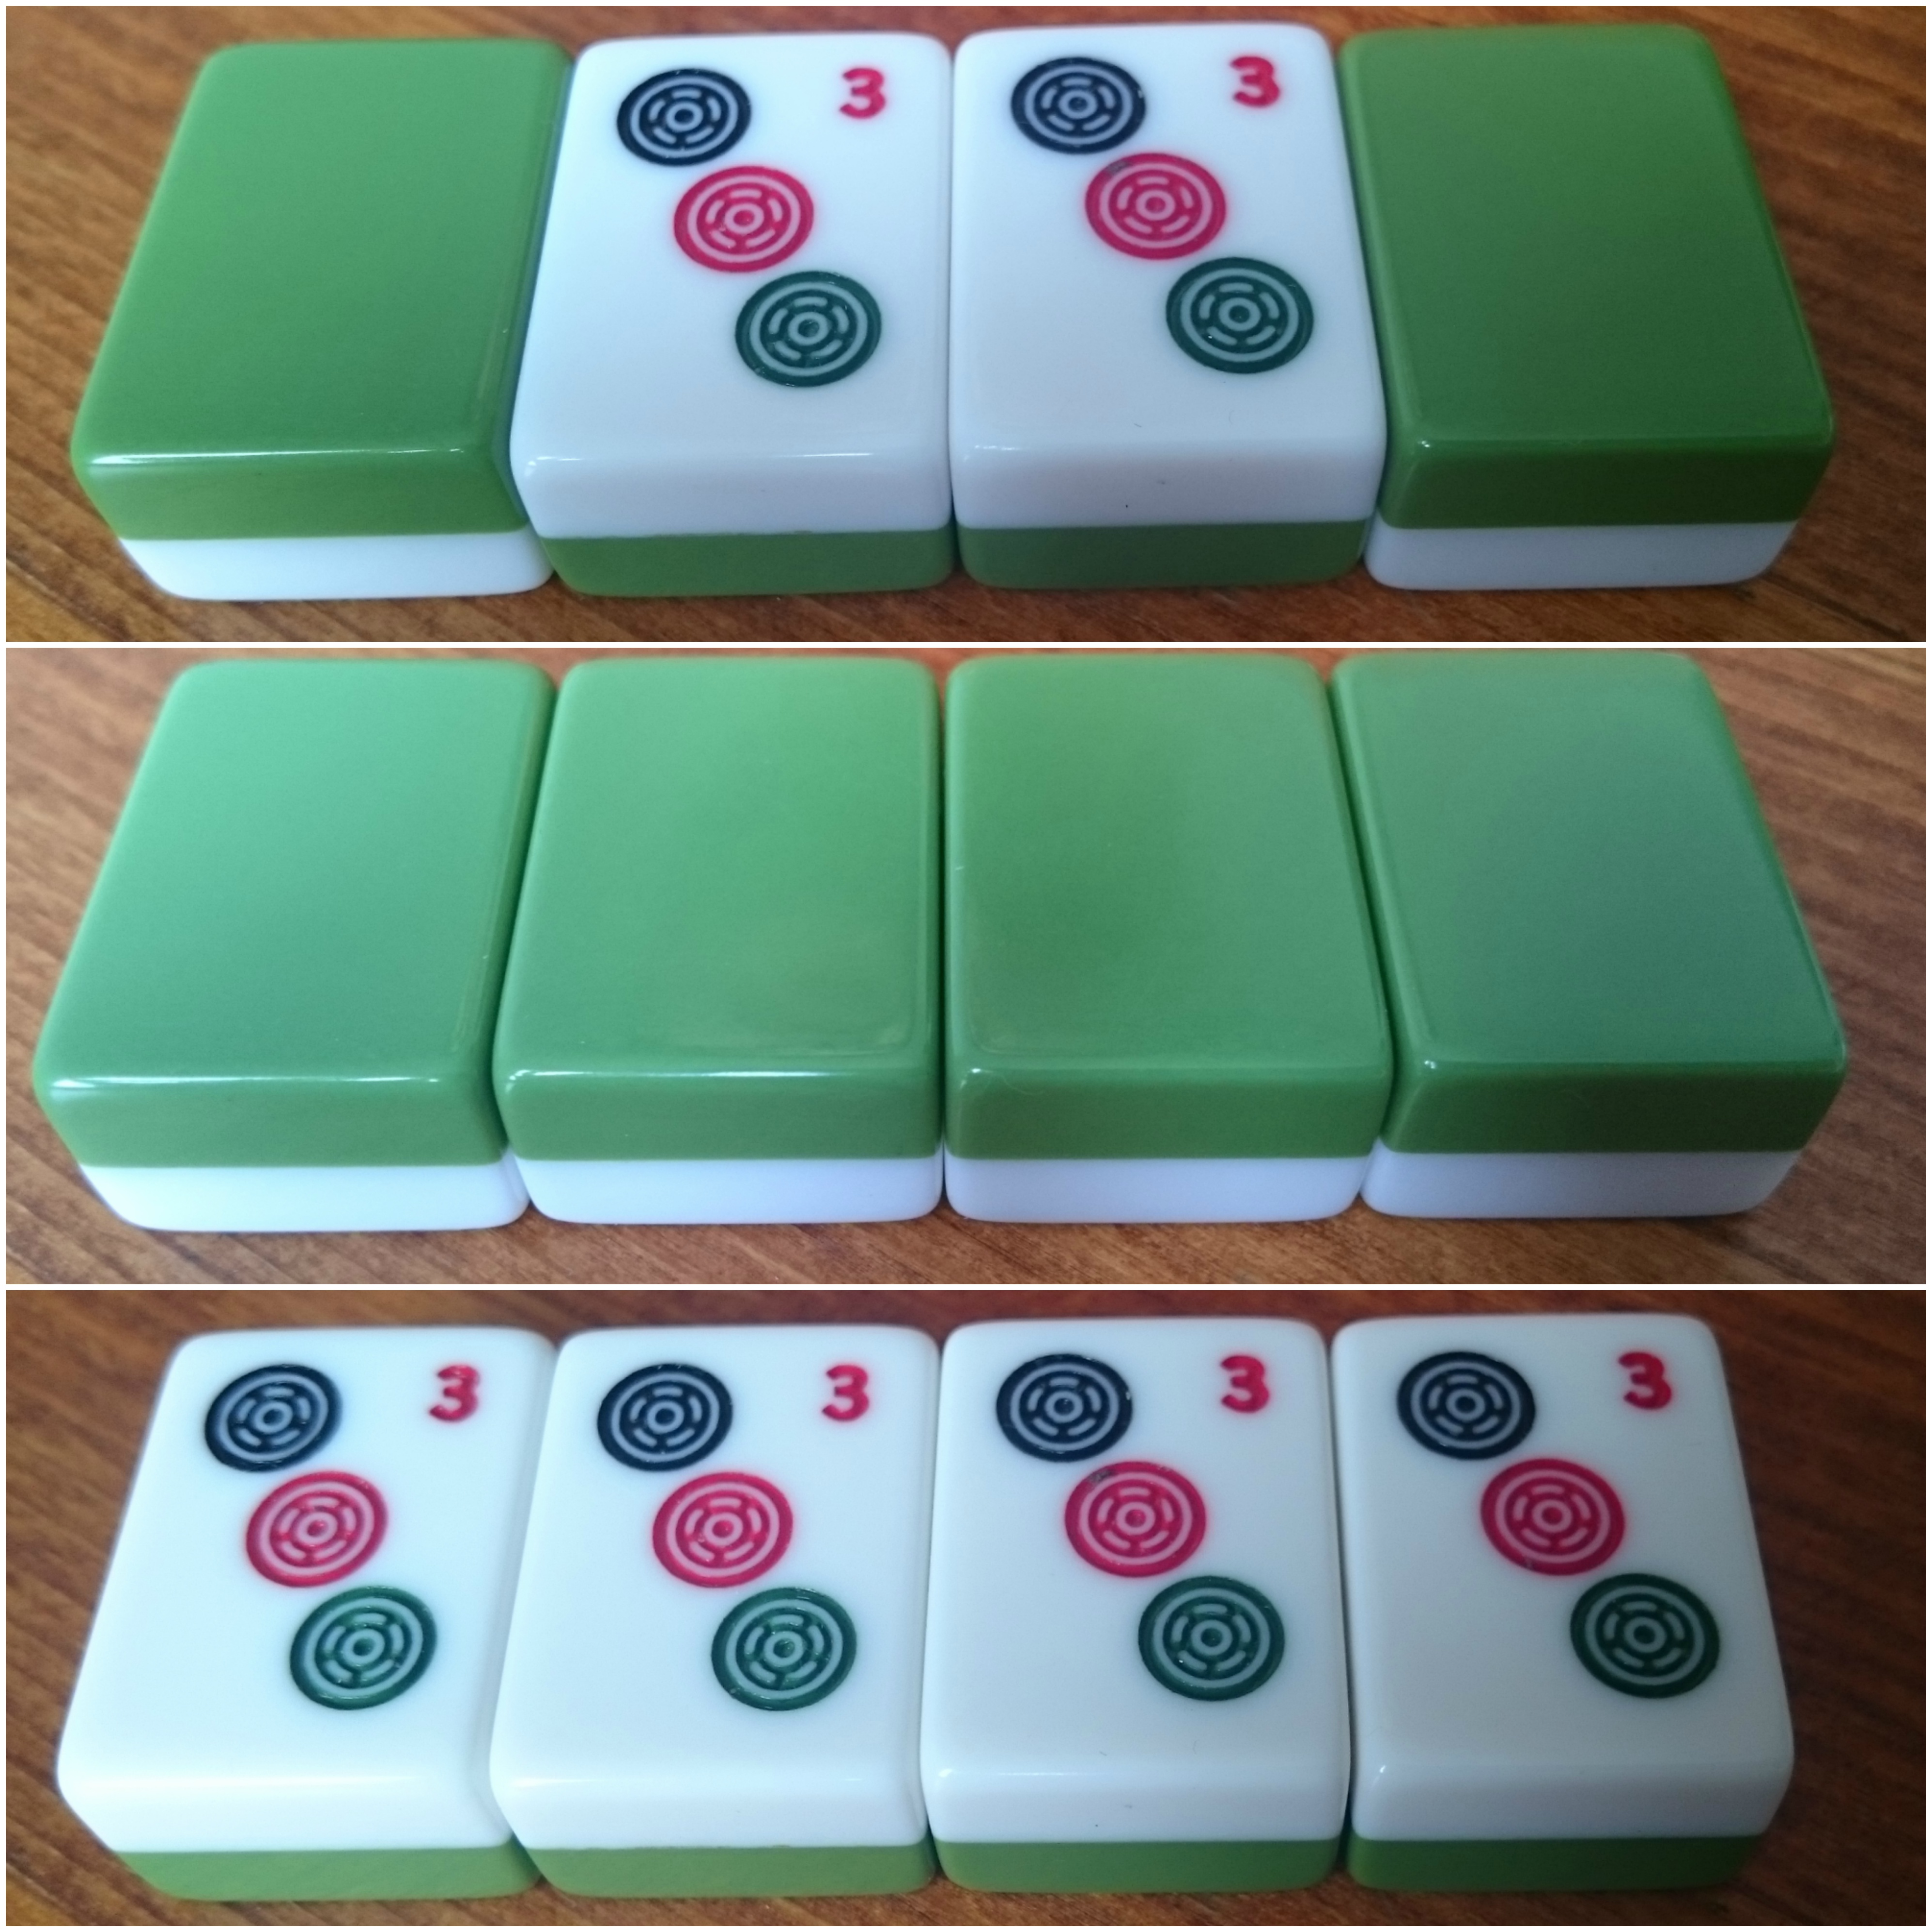
\includegraphics[width=0.50\textwidth]{gang_wariacje.jpg}
  \caption{3 możliwości oznaczania zamkniętego \pinyin{ganga}; kolejno od góry:
  w madżongu klasycznym i \romaji{rīchi}; w międzynarodowych zasadach
  turniejowych i w madżongu kantońskim; źródło: fotografia własna}
  \label{fig:closed_gang_options}
\end{figure}

Elementem wyróżniającym jest natomiast system liczenia punktów, który podobnie
jak międzynarodowe zasady turniejowe, oparty jest o \pinyin{fan} (jednakże
nie wszystkie układy i ich wartości są takie same - patrz też: strona
\pageref{fan}). Zsumowana wartość \pinyin{fan} jest traktowana jako wykładnik
potęgi liczby 2 przy liczeniu wartości punktowej ręki, zgodnie ze wzorem(S --
łączna wartość ręki; p - łączna wartość \pinyin{fan}):
	\begin{equation*}
		S = 2^{p}
		\label{hkos_scoring:point_score}
	\end{equation*}
Łączna wartość fan to wspomniana suma, zgodnie ze wzorem (f -- wartość danego
\pinyin{fan}; n -- liczba wszystkich \pinyin{fan}, które wystąpiły na
wygrywającej ręce):
	\begin{equation*}
		p = \sum\limits_{i=1}^n f_{i}
		\label{hkos_scoring:fan_score}
	\end{equation*}
(Lo 2001)

\subsection{Nowy styl}
Nowy styl wariantu kantońskiego to jego młodsza odmiana, która stała się
popularna po II Wojnie Światowej. Później, gdy w 1966 w Chińskiej Republice
Ludowej zakazano gry w madżonga, wielu udawało się do Hong Kongu tylko po to, by
móc grać - a nowy styl był tam najpopularniejszym zestawem zasad.

Już od początku rozgrywki widać wizualne różnice. Mur budowany jest w inny
sposób -- zamiast kłaść kamienie na sobie w 2 warstwach, są one umieszczane
równolegle obok siebie (lub w kształt ,,wiatraka'' -- patrz: Rysunek
\ref{fig:hkns_wall}).

\begin{figure}[H]
  \centering
  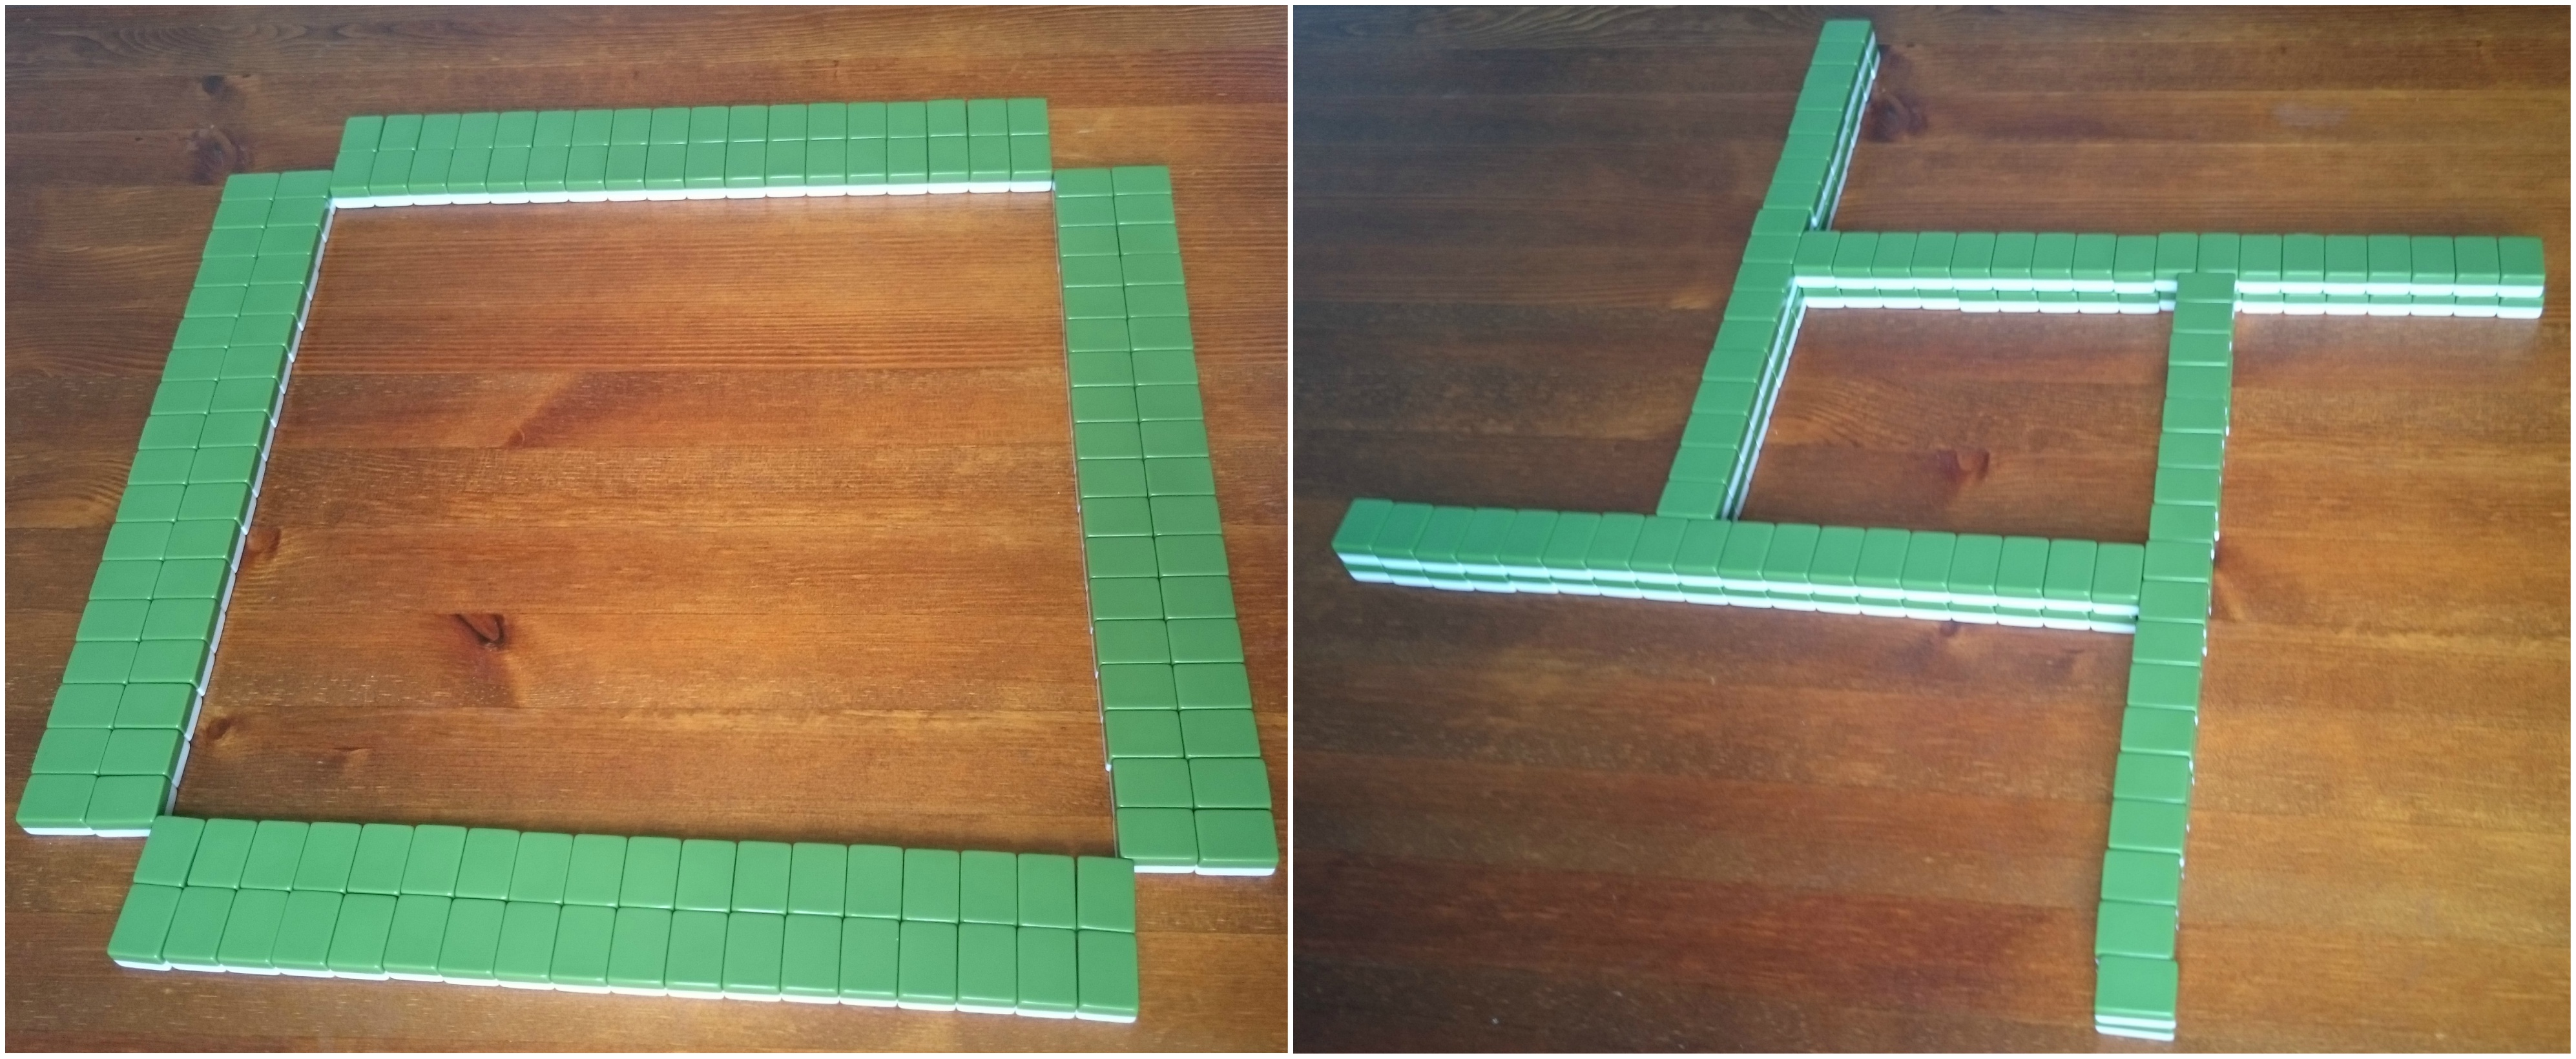
\includegraphics[width=0.8\textwidth]{hkns_wall.jpg}
  \caption{2 dopuszczalne możliwości budowania muru w nowym stylu madżonga
  kantońskiego; wariant płaski -- kamienie są najpierw
dobierane z wewnętrznego kręgu, a potem z zewnętrznego, naprzemiennie);
,,wiatrak'' -- wraz z postępem gry, mury są spychane do środka stołu, aby
kolejny kamień był łatwy do dobrania dla każdego z 4 graczy; źródło:
  fotografia własna}
  \label{fig:hkns_wall}
\end{figure}

Również przełamanie muru następuje w charakterystyczny sposób - wykonywany jest
tylko jeden rzut, lecz używa się do niego 3 (a nie 2) sześciennych kości.
Ponadto, dokonuje go gracz wschodni i żaden z pozostałych graczy nie bierze
udziału w tej czynności.

System liczenia punktów jest oparty o ten używany w starym stylu, jednakże
używany jest inny (większy) zbiór różnych \pinyin{fan} oraz wprowadzono w nim
limity -- \jyutping{laat} (辣 \jyutping{laat6}). Jako że madżong kantoński jest
grą hazardową, a punkty przeliczane są bezpośrednio na pieniądze, w kontekście
ilości różnych \pinyin{fan}, jakie naraz mogą znaleźć się w tym wariancie na
wygrywającej ręce, wysokie wygrane mogły potencjalnie przekraczać możliwości finansowe
przegranych uczestników gry. Z tego właśnie względu wprowadzono \jyutping{laat},
które pozwalają ograniczyć maksymalną możliwą wygraną. \pinyin{Fan} o łącznej
wartości 4, 5 lub 6 mają wartość 1 \jyutping{laat}, które przekłada się na 16 punktów
(czyli standardową wartość dla 4 \pinyin{fan}). 2 \jyutping{laat} to od 7 do 9
\pinyin{fan}, natomiast 3 \jyutping{laat} to 10 i więcej. W bardziej hazardowym
podwariancie można grać aż do 5 \jyutping{laat} (20 \pinyin{fan}), w czego
efekcie wartość ręki może osiągnąć nawet 2048 punktów, przez co przed grą
istotne jest ustalenie przez graczy, do którego limitu zamierzają grać (Rep 2006).

\section{Wiek madżonga klasycznego i kantońskiego}
\label{ccvshkos}
Niewątpliwie madżong klasyczny oraz kantoński w starym stylu sa najstarszymi
znanymi regułami gry, jednakże jest kwestią sporną, który z nich jest starszy
od drugiego. Argumenty za oboma potencjalnymi rozwiązaniami, które autor
przedstawia w dalszej części tej sekcji, pochodzą z zapisu dyskusji Toma
Slopera, Alana Kwaana i Cofa Tsui (Sloper i inni autorzy 2006).

Za starszeństwem zasad klasycznych przemawia fakt, że wszystkie źródła
pochodzące z lat dwudziestych XX wieku, kiedy zasady gry ulegały standaryzacji,
nie wspominają o wariancie kantońskim, nawet w kontekście Hong Kongu,
co jasno sugeruje, że wariant klasyczny mógł być wówczas jedynym istniejącym.
Ponadto, oba zestawy zasad są bardzo zbliżone w kwestii samego procesu gry,
różniąc się przede wszystkim sposobem liczenia punktów, który z kolei jest mniej
skomplikowany w przypadku madżonga kantońskiego -- z czego można wysunąć
wniosek, że jest on uproszczeniem wersji klasycznej.

Jako że madżong nie powstał od razu w swojej docelowej formie, lecz stanowił
rozwinięcie wielu istniejących wcześniej gier, problem jest tym bardziej
skomplikowany. Ponadto, Cofa Tsui argumentuje, że jest mało prawdopodobne, by w
tak wczesnym okresie rozwoju gry zasady były upraszczane -- naturalnym
kierunkiem rozwoju zasad jest proces odwrotny, co wskazywałoby na starszeństwo
reguł kantońskich.

Zasady kantońskie w przeciwieństwie do klasycznych nie przewidują, aby w
przypadku zwycięstwa w rozdaniu kiedykolwiek któryś z graczy poza wygranym
otrzymywał punkty -- co jest cechą wspólną z \pinyin{madiao} i innymi
protoplastami madżonga. 

Jednakże, zgodnie z badaniami Thierry'ego Depaulisa i Cofa Tsui, istnieje też
teoria, że w rzeczywistości wcześniej (pomiędzy powstaniem gry a 1920 rokiem)
mogło istnieć wiele innych, jeszcze nieustandaryzowanych i niejednolitych
zestawów zasad, z których mogły się wywodzić oba późniejsze warianty (zarówno
klasyczny, jak i kantoński) (Depaulis [\&] Tsui 2007).

\section{Madżong japoński}
Madżong pojawił się po raz pierwszy w Japonii w 1907 roku. Został przywieziony
przez japońskiego żołnierza nazwiskiem Hirayama Saburo, który wcześniej spotkał
się z nim w Chinach, a następnie w roku 1924 założył szkołę gry (w tym samym
roku miały miejsce pierwsze zawody na skalę ogólnokrajową). Według innej teorii
madżong dotarł do Japonii za pośrednictwem pisarza Natsume Sōseki
\footnote{Natsume Sōseki (夏目漱石, 1867-1916) -- jego prawdziwe imię to Kinnosuke (金之助); pisarz
japoński tworzący w epoce Meiji (明治).} -- madżong pojawił się w zapiskach z jego
podróży do Chin w 1909 roku. W ciągu kolejnych dekad nastąpił gwałtowny wzrost
popularności gry w Japonii, grywał w nią nawet sam cesarz Hirohito (裕仁)
(Kolenda 2012).

Madżong, podobnie jak znacznie wcześniej pismo chińskie, został przez
Japończyków zaadaptowany do ich potrzeb, zamiast być przyjętym w niezmienionej
postaci. Poza tym, że przy stole używana jest terminologia po japońsku (dla
przykładu, \romaji{kan} (槓 lub カン) zamiast \pinyin{gang}), zestaw do gry różni
się od tego stosowanego w innych wariantach gry. Kamienie kwiatów nie są używane
(większość japońskich zestawów jest ich w ogóle pozbawiona), natomiast
występują 3 unikalne, występujące w jednym egzemplarzu kamienie -- tak zwane
,,czerwone piątki'' lub ,,czerwone \romaji{dory}'' (赤牌 \romaji{akapai} lub 赤ドラ
\romaji{akadora}). Są to dodatkowe egzemplarze kamieni o numerze 5 w każdej z 3
talii, które od zwyczajnych różnią się pomalowanym na kolor czerwony wzorem.
Kamienie białego smoka również różnią się od chińskich - są to białe, gładkie
kamienie bez żadnego wzoru (podczas gdy chiński wzór to czarna lub niebieska
obwódka wokół prostokątnego kamienia) (Rep 2006).

Istnieją 2 główne odmiany madżonga japońskiego -- tradycyjny i \romaji{rīchi}
(立直 lub リーチ) (Kolenda 2012), jednakże ze względu na ogólnoświatową popularność
wariantu \romaji{rīchi} autor postanowił skupić na nim całą uwagę.
% 
% \subsection{Madżong japoński tradycyjny}
% \label{japanese_traditional}

\subsection{Madżong japoński \romaji{rīchi}}
\label{rīchi}
Madżong \romaji{rīchi} powstał w latach pięćdziesiątych XX wieku, kiedy grywali
w niego zawodowi hazardziści, którzy później przyczynili się do jego
popularyzacji. Jest on bardzo popularny nie tylko w Japonii, ale też na
całym świecie (Rep 2006). Jest to jeden z 2 wariantów zasad gry, zgodnie z
którym organizowane są turnieje Europejskiej Organizacji Mahjonga (drugi to
międzynarodowe zasady turniejowe) (European Mahjong Association 2016) oraz
jedyny, w którym organizowane są turnieje w Polsce (Polska Liga Mahjonga 2016).
Znajdujące się w dalszej części tej sekcji wyjaśnienie wyróżniających elementów
jego zasad zostało wykonane na podstawie aktualnej wersji reguł obowiązujących
na zawodach Europejskiej Organizacji Mahjonga (European Mahjong Association
2016), ich poprzedniej edycji z roku 2012 (European Mahjong Association 2012)
oraz książki \textit{The Great Mah Jong Book: History, Lore, and Play} (Rep
2006). Używana terminologia oparta jest o tę używaną przez Polską Ligę Mahjonga
(Polska Liga Mahjonga 2016).

Istotną częścią zestawu do gry w \romaji{rīchi} są  \romaji{tenbō} (点棒) --
liczmany służące nie tylko do oznaczania posiadanej liczby punktów, ale są też
potrzebne do niektórych sytuacji w grze. Niejako podkreślają też hazardowe
pochodzenie gry, jako że mogą nasuwać skojarzenia z żetonami używanymi w grach
takich jak poker.

Budowa muru na początku rozgrywki jest zbliżona do wariantu \foreign{Mixed-Hand}
zasad chińskich klasycznych (patrz: strona \pageref{cc_mixed_hand}) --
występuje martwy mur składający się ze stałej liczby 14 kamieni. Gdy dobrany
zostanie kamień uzupełniający (嶺上牌 \romaji{rinshanpai} -- dosłownie ,,kamień ze
szczytu góry''), dokładany jest dodatkowy kamień z końca zwykłego muru aby
zachować stałą liczbę kamieni -- w ten sposób dobranie kamienia uzupełniającego
nie wydłuża faktycznie rozgrywki.

Elementem charakterystycznym dla \romaji{rīchi}, którego oznaczenie znajduje się
także w budowie martwego muru, jest \romaji{dora} (ドラ) -- specjalny, losowy w
każdym rozdaniu kamień, którego każde wystąpienie na wygrywającej ręce zwiększa
znacząco jej wartość punktową. To, który kamień jest \romaji{dorą} w danym
rozdaniu, zależy od jej indykatora -- trzeciego kamienia od końca martwego muru.
Jest on odkrywany po zbudowaniu muru, a kamień o wartości o jeden wyższej od
indykatora jest \romaji{dorą} w tym rozdaniu. Ponadto, każda deklaracja
\pinyin{ganga} w rozdaniu wiąże się z odkryciem kolejnego indykatora po jego
lewej stronie, w efekcie czego naraz może być w grze 5 różnych \romaji{dor},
jako że nie jest dozwolone zadeklarowanie więcej niż 4 \pinyin{gangów} w jednym
rozdaniu (patrz: Rysunek \ref{fig:rīchi_dead_wall}).

\begin{figure}[H]
  \centering
  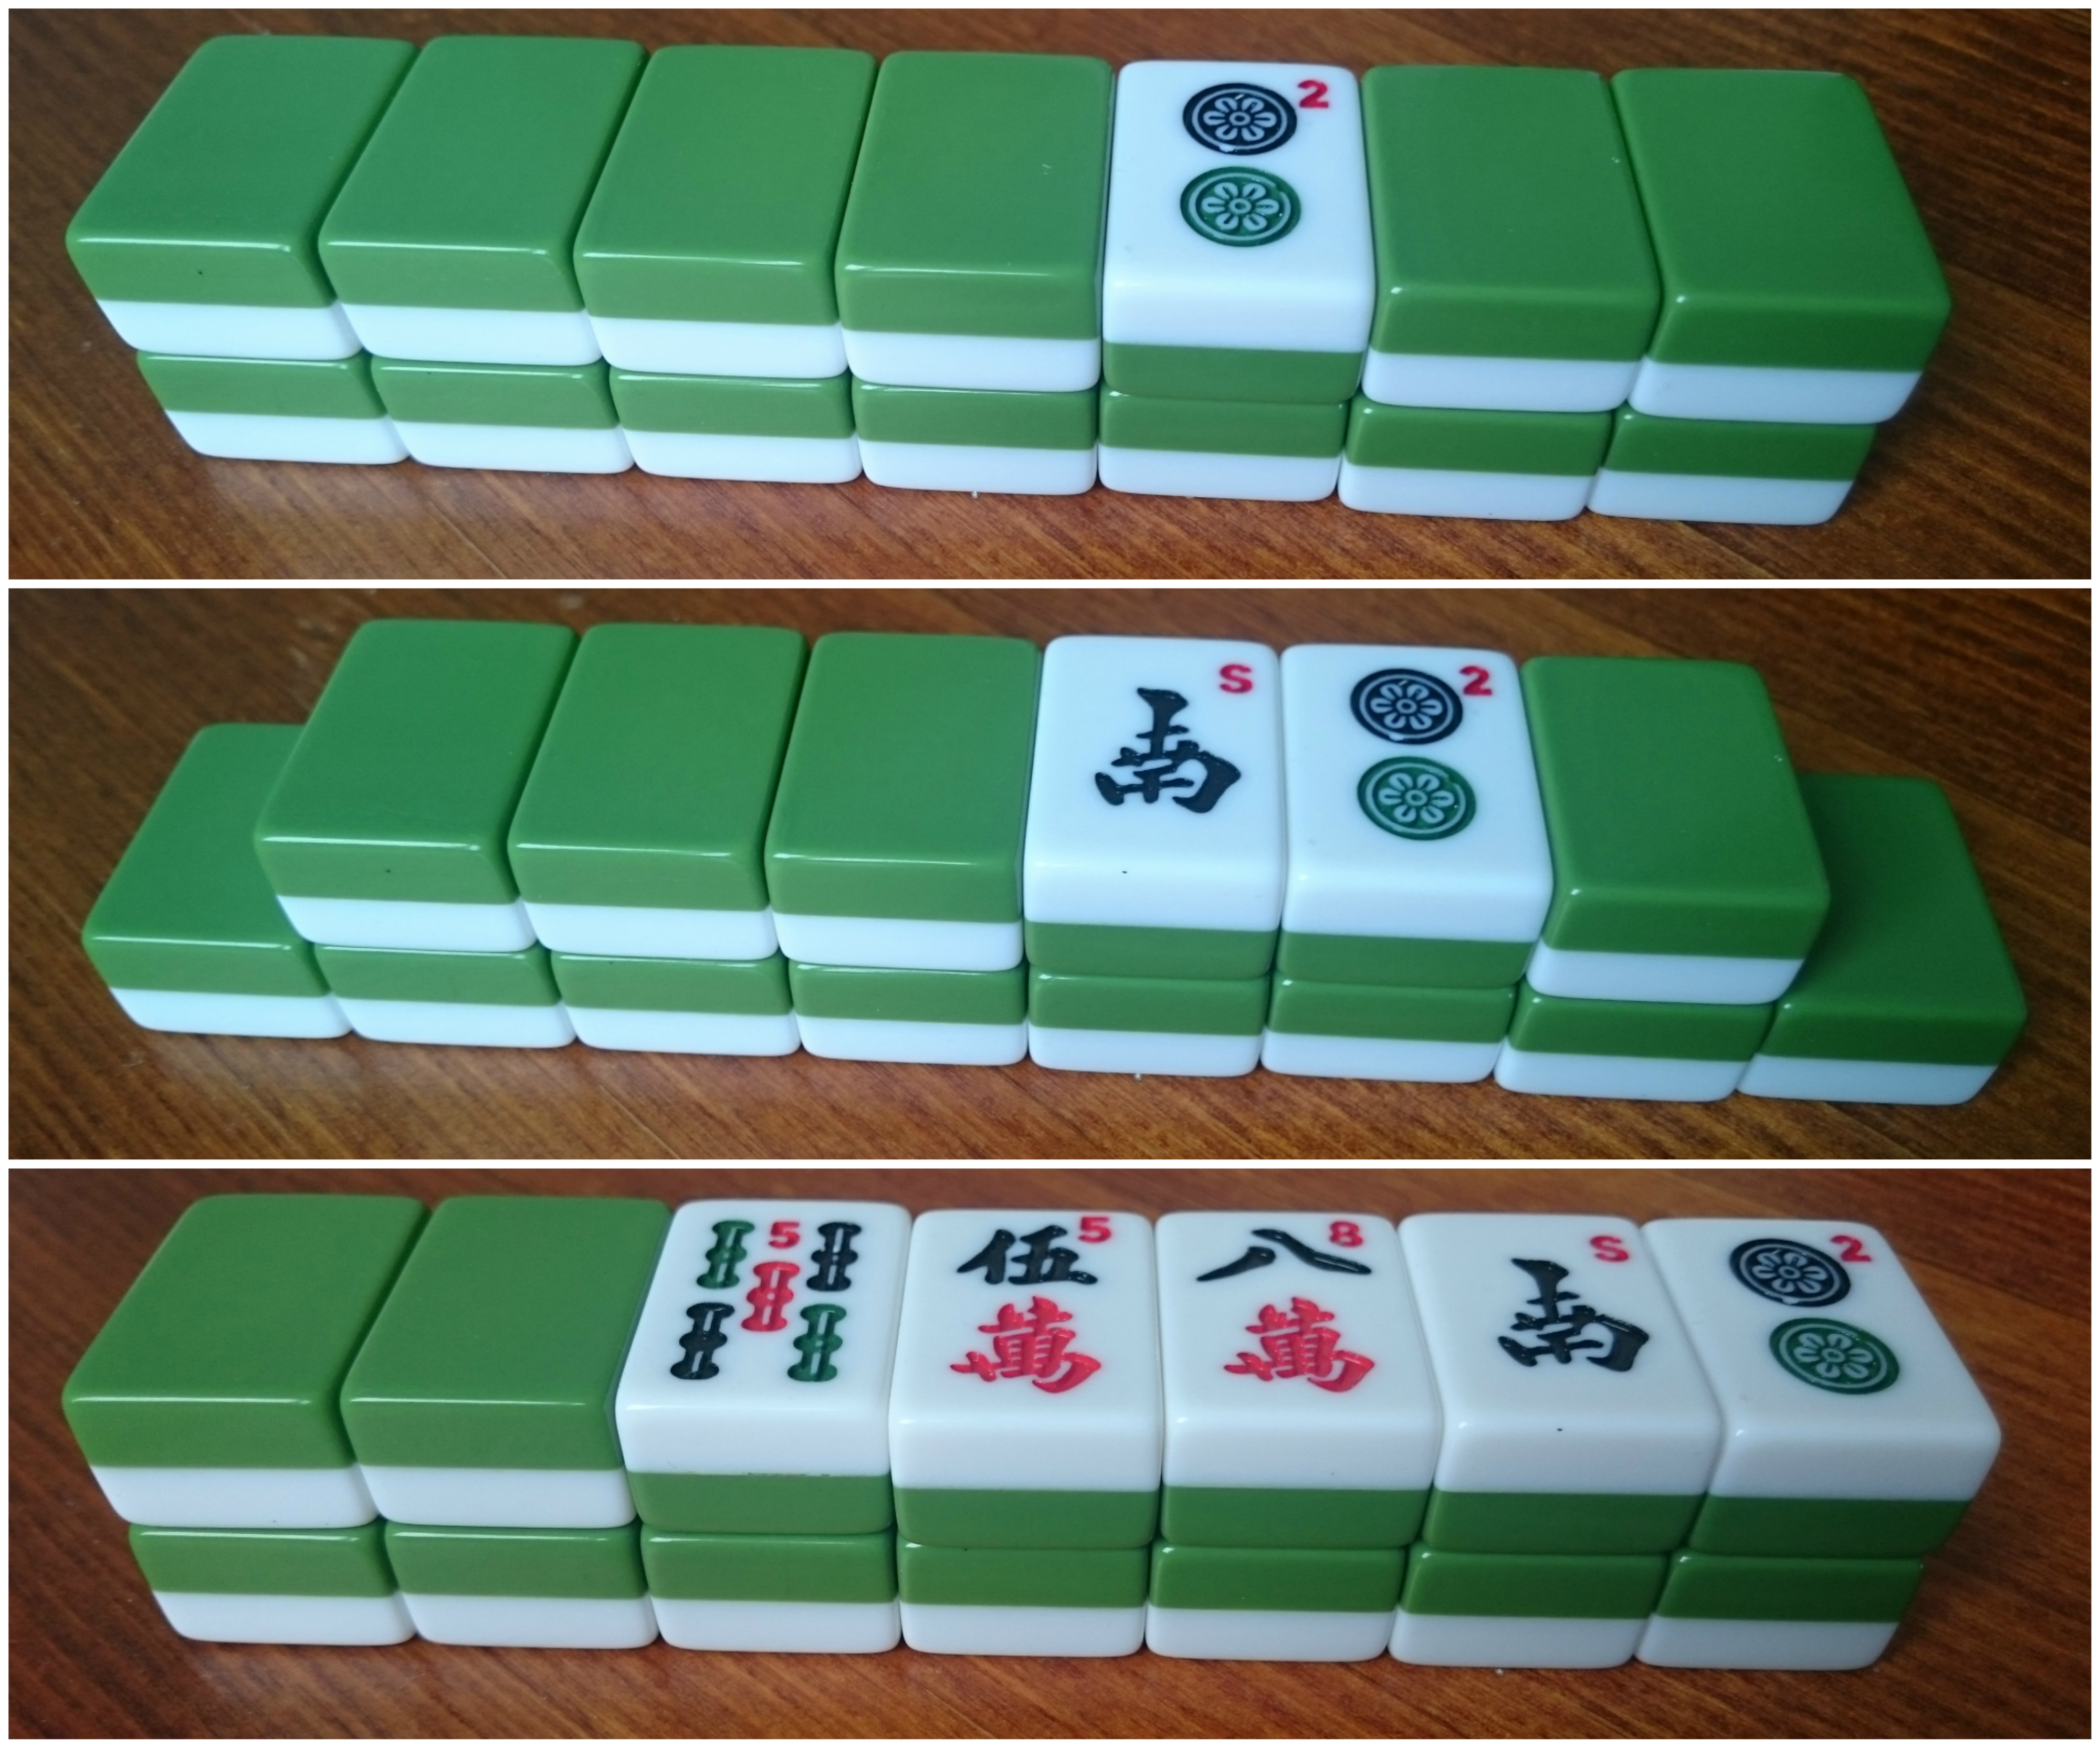
\includegraphics[width=0.5\textwidth]{riichi_dead_wall.jpg}
  \caption{Martwy mur w madżongu japońskim \romaji{rīchi}; indykatorami
  \romaji{dory} są odkryte kamienie, natomiast po ich prawej stronie
  znajdują się kamienie uzupełniające (maksymalnie 4); pierwsza fotografia
  przedstawia stan na początku rozdania, druga -- po deklaracji 1
  \pinyin{ganga}, a trzecia -- po deklaracji wszystkich 4 możliwych
  \pinyin{gangów}; na przykładzie pierwszej fotografii, indykatorem
  \romaji{dory} jest 2 z talii kółek, więc \romaji{dorą} jest 3 z tej samej
  talii; źródło: fotografia własna}
  \label{fig:rīchi_dead_wall}
\end{figure}

Opcjonalną zasadą jest używanie wspomnianych wcześniej czerwonych \romaji{dor}
-- wówczas w każdej talii 1 z 4 kamieni o numerze 5 jest pomalowany wyłącznie
kolorem czerwonym. Czerwone \romaji{dory} są traktowane na
wygrywającej ręce identycznie jak zwykłe. Choć czerwone piątki są standardowym
elementem zestawów do japońskiego madżonga, nie są używane w aktualnej (z 2016
roku) wersji zasad Europejskiej Organizacji Madżonga (jednakże obowiązywały w
wersji z 2012 roku).

Kolejnym elementem charakterystycznym \romaji{rīchi} jest zasada, od której
pochodzi nazwa tego wariantu. \romaji{Rīchi} to specjalna deklaracja dozwolona
wtedy, gdy gracz znajdzie się w stanie czekania (określanym \romaji{tenpai}
(聴牌)) na zakrytej ręce. Wówczas poprzez tę deklarację może zastawić tysiąc
swoich punktów (kładąc odpowiednie \romaji{tenbō} na stół) i umieścić
odrzucony kamień poziomo. Od tego momentu gracz nie może już wykonywać innych
deklaracji (nie licząc zakrytego \pinyin{ganga}, o ile nie zmienia on kamieni,
na które oczekuje gracz) ani zmieniać składu swojej ręki, jednakże wartość
punktowa jego ręki w przypadku wygranej się zwiększy (w przypadku przegranej
1000 punktów, które zostało położone w zastaw na stole, zostaje utracone).

Występuje szereg pomniejszych wyróżniających zasad odróżniających \romaji{rīchi}
od innych wariantów madżonga (zakryty \pinyin{gang} oznaczany jest tak, jak w
zasadach chińskich klasycznych, występuje ścisłe rozróżnienie deklaracji
zwycięstwa na odrzuconym kamieniu oraz na kamieniu dobranym z muru, a także
inne), jednakże pozostałe elementy gry są bardzo zbliżone do madżonga
kantońskiego w nowym stylu. Informacje o odrzuconych kamieniach są zachowywane
na stole, identycznie jak w wyżej wymienionym wariancie, jak też i w
międzynarodowych zasadach turniejowych, jednakże rotacja miejsc na końcu rund
upodabnia te zasady do reguł hongkońskich.

Również system punktacji nasuwa bliskie skojarzenia z zasadami kantońskimi.
Występują limity podobne do \jyutping{laat} przy konkretnych wartościach
punktowych, przy czym każdy z nich ma swoją własną nazwę. 
% (\romaji{mangan},
% \romaji{haneman}, \romaji{baiman}, \romaji{sanbaiman} i \romaji{yakuman})
Istnieją 2 pośrednie rodzaje punktów:
\begin{itemize}
  \item \romaji{han} (飜) -- wartości konkretnych \pinyin{fan}, zwanych w
  madżongu japońskim \romaji{yaku} (役);
  \item \romaji{fu} (符) -- liczone są w bardzo podobny
sposób do punktów podstawowych w madżongu chińskim klasycznym, jak też i pełnią
podobną rolę, będąc wartością mnożoną przez konkretną potęgę liczby 2.
\end{itemize}
Punkty (nie licząc sytuacji, gdy przekraczają któryś z 5 istniejących w
zasadach limitów i są ustaloną wartością) są liczone z następującego wzoru (S
-- łączna wartość punktowa wygrywającej ręki; Fu -- liczba punktów \romaji{fu};
Han -- liczba punktów \romaji{han}):

	\begin{equation*}
		S = Fu \times 2^{2 + Han}
		\label{rīchi_scoring}
	\end{equation*}
	
W przypadku zwycięstwa na kamieniu odrzuconym przez innego gracza, ów gracz jest
odpowiedzialny w pełni za wypłatę wygranej, co narzuca konieczność rozwagi przy
odrzucaniu kamieni (jako że można spowodować nie tylko cudzą wygraną, ale także
utratę własnych punktów) i często -- grę defensywną. Ponadto, wiele
obowiązujących \romaji{yaku} narzuca konieczność posiadania zakrytej ręki, przez
co deklaracje na kamieniach odrzuconych przez innych graczy do własnych zestawów
często nie są tak opłacalne, jak byłoby w innych wariantach zasad.

Mimo że \romaji{rīchi} jest jednym z najbardziej skomplikowanych wariantów, jest
ceniony na całym świecie za swoją dynamikę gry wprowadzaną przez unikalne dla
niego zasady. 

 %Lo 2001
%TODO: klasyczny/HK - który starszy
%	\label{ccvshkos}
%TODO: hong kong new style
%	\label{hkns}
%TODO: japoński rīchi
%TODO: amerykański
%TODO: opcjonalne:
% - tajwański
% - koreański
% - singapurski


\printindex
\onecolumn
\section*{Bibliografia}
\setlength{\parindent}{0pt}
\setlength{\parskip}{1ex plus 0.5ex minus 0.2ex}
Babcock, Joseph P. [\&] Foster, R. F. [\&] Hartman, Lee F. [\&] Smith, John H.
[\&] Work, Milton C. 1924. ,,The American Code Of Laws For Mah-Jongg'' W:
\textit{Mah-Jongg Up-To-Date}. The John C. Winston Company. 
% brak stron imminent
%\\https://groups.google.com/forum/\#!msg/rec.games.mahjong/lTDLqLLykFY/g00IBFra\_skJ
% [dostęp 2016-08-01]


Carlisle, Rodney P. 2009. ,,Mahjong'' W: \textit{Encyclopedia of Play in Today's
Society}, 371-372.
Sage Publications.

Culin, Stewart 1924. ,,The Game of Ma-Jong'' W: \textit{Brooklyn Museum
Quarterly}, Volume XI, 153-168.

Depaulis, Thierry [\&] Tsui, Cofa 2007. \textit{Evolution of Various Forms of
Mahjong (1890-2001)}. 
\\http://www.imahjong.com/maiarchives205d\_3.html [dostęp
2016-08-01]

European Mahjong Association 2012. \textit{\romaji{Riichi} -- Rules for Japanese Mahjong}.
\\http://mahjong-europe.org/docs/riichi\_EN.pdf [dostęp 2016-08-05]

European Mahjong Association 2016. \textit{\romaji{Riichi} -- Rules for Japanese Mahjong}.
\\http://mahjong-europe.org/docs/Riichi-rules-2016-EN.pdf [dostęp 2016-08-05]

Greenfield, Mary C. 2010. „The Game of One Hundred Intelligences: ,,Mahjong,
Materials, and the Marketing of the Asian Exotic in the 1920s''. W:
\textit{Pacific Historical Review}, Vol. 79. 329-359.
% Carl Abott i David A. Johnson (ed.), \textit{Pacific Historical Review}, Vol.
% 79. 329-359. California: University of California Press.

Harr, Lew Lysle 2008. \textit{Pung Chow -- The Game of a Hundred Intelligences.
Also known as Mah-Diao, Mah-Jong, Mah-Cheuk, Mah-Juck and Pe-Ling}. Project
Gutenberg

Jīn Xuéshī 金学诗 1783. \textit{Mùzhū Xiánhuà 牧猪闲话 [Plotki o Świniopasach]}.
\pinyin{Zhāodài} \pinyin{Cóngshū} 昭代丛书

Kanazawa Masahiro 金澤正浩 2010. \romaji{,,2002 Sekaimājansenshuken taikai ni
tsuite''} 《2002 世界麻雀選手権大会について》 (\textit{O Światowych Mistrzostwach
Świata w Madżongu 2002}).
\\http://www1.tcue.ac.jp/home1/takamatsu/100124/100124-002.pdf [dostęp
2016-04-25]

Kolenda, Dominik 2012. \textit{Mahjong w japońskiej kulturze popularnej --
Historia: Japonia}. Polska Liga Mahjonga.
\\https://mahjong.waw.pl/index.php?option=com\_content\&view=article\&id=11\&Itemid=128
[dostęp 2016-08-06]

\pinyin{Kǒuzhuāng Bāshì} 口装巴士 2014. \pinyin{,,Huānlè májiàng
yánshēn zhī shìjiè májiàng bǐsài jièshào''} 《乐麻将延伸之世界麻将比赛介绍》
(\textit{Popularyzacja madżonga poprzez wprowadzenie światowych zawodów
sportowych}) \\http://m.ptbus.com/huanlemajiang/221298/ [dostęp 2016-04-25]

Lo, Amy 2001. \foreign{The Book of Mah jong: An Illustrated Guide}. Tuttle
Publishing

Mah Jong Museum. \textit{Mah Jong Historical Documents}
\\http://www.mahjongmuseum.com/history.htm [dostęp
2016-03-30]

Miller, Scott D. 2015. \textit{Riichi Mahjong: The Ultimate Guide to the
Japanese Game Taking the World By Storm}. Psionic Press.

\romaji{Nihon kenkō asa shō kyōkai kōshiki saito} 日本健康麻将協会公式サイト  2002.
\\\romaji{2002 nen Sekaimājansenshuken Taikai Kojin Bumon Seiseki} 2002 年世界麻雀選手権大会個人部門成績 (Wyniki
Indywidualne Światowych Zawodów Madżonga 2002)
\\http://www.kenko-mahjong.com/topics/sekaikojin.htm [dostęp 2016-04-25]

Polska Liga Mahjonga 2016. \textit{Terminologia}
\\
https://mahjong.waw.pl/index.php?option=com\_content\&view=article\&id=24\&Itemid=147
[dostęp 2016-07-12]

Polska Liga Mahjonga 2016a. \textit{Turnieje PLM -- System turniejowy Polskiej
Ligi Mahjonga} \\https://turnieje.mahjong.waw.pl/ [dostęp 2016-08-06]

Rep, Jelte 2006. \textit{The Great Mahjong Book: History, Lore, and Play}.
Tuttle Publishing. %hkns 129-142

Sina \pinyin{Xīnlàng Lùntán} 新浪论坛 2010. \pinyin{Zhùmíng xuézhě Yú Guāngyuǎn,
wǎnnián wèishénme} \\\pinyin{qīngxīn hóngyáng májiàng wénhuà}
《著名学者于光远,晚年为什么倾心弘扬麻将文化》(\textit{Dlaczego szanowany uczony Yu Guangyuan na
starość całym sercem promuje kulturę gry w madżonga})
\\http://club.history.sina.com.cn/thread-4268500-1-1.html [dostęp 2016-06-27]

\pinyin{Shìjiè Májiàng Zǔzhī} 世界麻将组织 2014. \pinyin{Májiàng Jìngsài
Guīzé}《麻将竞赛规则》 (\textit{Światowe Zasady Madżonga})
\\http://www.chinamajiang.com/adobe\%20reader/z20140402.pdf [dostęp 2016-01-04]

Sloper, Tom [\&] inni autorzy 2006. \textit{The CC Theory}
\\http://www.sloperama.com/cctheory/detail.html [dostęp
2016-03-30]

Sloper, Tom 2002. \textit{Identifying a Mah-Jongg Variant}
\\http://www.sloperama.com/mjfaq/mjfaq02b.html [dostęp
2016-06-27]

Sloper, Tom 2006. \textit{History of Mahjong}
\\http://www.sloperama.com/mjfaq/mjfaq11f.htm [dostęp 2016-08-01]

% TODO: rozróżnić a, b z różnych publikacji i tych samych lat
Stanwick, Michael 2004. ,,Mahjong(g) Before Mahjong(g): Part 1''. W:
\textit{The Playing-card}, Vol. 32, No. 4, 153-162

Stanwick, Michael 2004a. ,,Mahjong(g) Before Mahjong(g): Part 2''. W:
\textit{The Playing-card}, Vol. 32, No. 5, 206-215
% \\http://www.themahjongtileset.co.uk/tile-set-history/mahjongg-before-mahjongg-part-1/ 
% \\http://www.themahjongtileset.co.uk/tile-set-history/mahjongg-before-mahjongg-part-2/
% [dostęp
% 2016-03-30]

Stanwick, Michael 2006. ,,Mahjong(g) Before and After Mahjong(g): Part 1''. W:
\textit{The Playing-card}, Vol. 34, No. 4, 259-268

Stanwick, Michael 2006a. ,,Mahjong(g) Before and After Mahjong(g): Part 2''. W:
\textit{The Playing-card}, Vol. 35, No. 1, 27-39

% Stanwick, Michael 2006. \textit{Mahjong(g) Before And After Mahjong(g)}
% %\\http://www.themahjongtileset.co.uk/tile-set-history/mahjongg-before-and-after-mahjongg-part-1/
%  \\http://www.themahjongtileset.co.uk/tile-set-history/mahjongg-before-and-after-mahjongg-part-2/
% [dostęp
% 2016-03-30]

Stanwick, Michael [\&] Xu, Hongbing 2012. ,,From Cards to Tiles: The Origin of
Mahjong(g)’s Earliest Suit Names''. W:\textit{The Playing-card}, Vol. 41, No. 1,
52–67.

Stanwick, Michael [\&] Xu, Hongbing. \textit{Mahjong terms 1780 – 1920}
\\http://www.themahjongtileset.co.uk/mahjong-terms-1780-1920/ [dostęp
2016-03-30]

Tse, Samson [\&] Yu, Alex C.H. [\&] Rossen, Fiona [\&] Wang, Chong-Wen
2010.
,,Examination of Chinese Gambling Problems through a Socio-Historical-Cultural Perspective''. W: \textit{The
Scientific World Journal}

%Stanwick, Michael; Xu, Hongbing. \textit{From Cards to Tiles: The Origin of
% Mahjong(g)’s Earliest Suit Names}
%\\http://www.themahjongtileset.co.uk/tile-set-history/earliest-suit-names/
Wikipedia 2013. \textit{George B. Glover}
\\https://en.wikipedia.org/wiki/George\_B.\_Glover [dostęp 2016-04-22]

Wikipedia 2016. \textit{Stewart Culin}
\\https://en.wikipedia.org/wiki/Stewart\_Culin [dostęp 2016-04-22]

Wikipedia 2016a. \textit{Yú Guāngyuǎn} 于光远
\\https://zh.wikipedia.org/wiki/\%E4\%BA\%8E\%E5\%85\%89\%E9\%81\%A0 [dostęp
2016-06-27]

% Work, Milton C. 1924. \textit{Mah-Jongg Up-To-Date}. The John C. Winston
% Company.

World Heritage Encyclopedia 2014. \textit{Mahjong}
\\http://www.worldheritage.org/article/WHEBN0000019496/Mahjong [dostęp
2016-03-31]

World Series of Mahjong 2015. \textit{Mahjong Around the World}
\\http://worldmahjong.com/about-mahjong/mahjong-around-the-world/ [dostęp
2016-06-27]

Zǐ Mò 梓沫 2015. \pinyin{,,Cáipàn jiědú guóbiāo májiàng: Bā
fān qǐ ‘hé’ jiàngdī yùnqì chéngfèn''}《裁判解读国标麻将:八番起‘胡’降低运气成分》
(\textit{Interpretacja sędziego krajowego madżonga:
hu przy 8 fan zmniejsza szczęście}) % tutaj jest o nowych zasadach z 1998
\\http://sports.sina.com.cn/go/2015-10-25/doc-ifxizwsi5588602.shtml [dostęp 2016-04-25]




% Please add the following required packages to your document preamble:
% \usepackage{multirow}
%\fan{Wielkie Cztery Wiatry}{大四喜}{Dà Sì Xǐ}{Trójki lub \pinyin{gangi} z każdego z 4 kamieni wiatrów.}
\section*{Suplement}
\tiny
\label{tab:fan2}
\begin{longtable}[]{|c|c|c|}
\caption{81 układów \pinyin{fan}} \\
%
%\hline
%\multicolumn{3}{|c|}{\centering 81 układów \pinyin{fan}}                       
% \\
\hline \multicolumn{1}{|c|}{Punkty} & \multicolumn{1}{c|}{Nazwa} & \multicolumn{1}{c|}{Opis} \\ \hline
\endfirsthead
\caption{c.d. 81 układów \pinyin{fan}} \\
%\hline
%\multicolumn{3}{|c|}{\centering 81 układów \pinyin{fan}}                       
% \\
\hline \multicolumn{1}{|c|}{Punkty} & \multicolumn{1}{c|}{Nazwa} & \multicolumn{1}{c|}{Opis} \\ \hline
\endhead
\hline
\caption{(\pinyin{Shìjiè Májiàng Zǔzhī} 2014)} 
\endfoot
\multirow{7}{*}{88}    &  \fan{Wielkie Cztery Wiatry}{大四喜}{Dà Sì Xǐ}        
					   &  Trójki lub \pinyin{gangi} z każdego z 4 kamieni wiatrów.                
					   \\ \cline{2-3} 
                       &  \fan{Wielkie Trzy Smoki}{大三元}{Dà Sān Yuán}                     
                       &  Trójki lub \pinyin{gangi} z każdego z 3 kamieni smoków.                   
                       \\ \cline{2-3} 
                       &  \fan{Wszystko Zielone}{绿一色}{Lǜ Yī Sè}                     
                       &  \tabsplit{Ręka złożona tylko i wyłącznie z ,,zielonych'' kamieni:}{2, 3, 4, 6 i 8 z talii bambusów oraz zielonych smoków.}                    
                       \\ \cline{2-3} 
                       &  \fan{Dziewięć Bram}{九莲宝灯}{Jiǔ Lián Bǎo Dēng}                     
                       &  \tabsplit{Kombinacja kamieni 1, 1, 1, 2, 3, 4, 5, 6, 7, 8, 9, 9, 9 w jednej talii}{(odchodzi od standardowej struktury ręki).}                    
                       \\ \cline{2-3} 
                       &  \fan{Cztery \pinyin{Gangi}}{四杠}{Sì Gāng}                   
                       &  Dowolna reka zawierająca 4 \pinyin{gangi}.               
                       \\ \cline{2-3} 
                       &  \fan{Siedem Kolejnych Par}{连七对}{Lián Qī Duì}                     
                       &  Siedem par kolejnych kamieni w jednej talii (odchodzi od standardowej struktury ręki).                     
                       \\ \cline{2-3} 
                       &  \fan{Trzynaście Sierot}{十三幺}{Shísān Yāo}                     
                       &  \tabsplit{Po jednym kamieniu z każdego z honorów oraz kamieni 1 i 9 z każdej z talii,}{a także jeden duplikat dowolnego z wymienionych.}                     
                       \\ \hline
\multirow{6}{*}{64}    &  \fan{Same Terminalne}{清幺九}{Qīng Yāo Jiǔ}                        
					   &  Cała ręka złożona tylko i wyłącznie z kamieni terminalnych.                 
					   \\ \cline{2-3} 
                       &  \fan{Małe Cztery Wiatry}{小四喜}{Xiǎo Sì Xǐ}                        
                       &  Ręka zawierająca 3 trójki (lub \pinyin{gangi}) z 3 wiatrów oraz parę z czwartego.                     
                       \\ \cline{2-3} 
                       &  \fan{Małe Trzy Smoki}{小三元}{Xiǎo Sān Yuán}                        
                       &  Ręka zawierająca 2 trójki lub \pinyin{gangi} z 2 smoków oraz parę z trzeciego.                     
                       \\ \cline{2-3} 
                       &  \fan{Same Honory}{字一色}{Zì Yī Sè}                        
                       &  Ręka złożona z samych honorów.                    
                       \\ \cline{2-3} 
                       &  \fan{Cztery Zakryte Trójki}{四暗刻}{Sì Ànkè}                        
                       &  Ręka zawierająca 4 zakryte trójki (lub \pinyin{gangi}).                     
                       \\ \cline{2-3} 
                       &  \fan{Czyste Terminalne Sekwensy}{一色双龙会}{Yīsè Shuānglónghuì}                        
                       &  Ręka złożona z 2  identycznych sekwensów 1, 2, 3 oraz 7, 8, 9, a także pary z 5, wszystko w jednej talii.                      
                       \\ \hline
\multirow{2}{*}{48}    &  \fan{Poczwórny Sekwens}{一色四同顺}{Yīsè Sì Tóngshùn}                        
					   &  Ręka zawierająca 4 egzemplarze identycznego sekwensu w tej samej talii.                    
					   \\ \cline{2-3} 
                       &  \fan{Kolejne Cztery\\Czyste Trójki}{一色四节高}{Yīsè Sì Jiégāo}                           
                       &  Ręka zawierająca 4 trójki lub \pinyin{gangi} 4 kolejnych kamieni w jednej talii.                     
                       \\ \hline
\multirow{3}{*}{32}    &  \fan{Kolejne Cztery\\Czyste Sekwensy}{一色四步高}{Yīsè Sì Bù Gāo}                     
					   &  \tabsplit{Ręka zawierająca 4 sekwensy w jednej talii, w których rozpoczynające je (najniższe) kamienie są 4 kolejnymi,}{odległymi od siebie o 1 lub 2.}                     
					   \\ \cline{2-3} 
                       &  \fan{Trzy \pinyin{Gangi}}{三杠}{Sān Gāng}                        
                       &  Ręka zawierajaca trzy \pinyin{gangi}.                     
                       \\ \cline{2-3} 
                       &  \fan{Same Terminalne i Honory}{混幺九}{Hùn Yāo Jiǔ}                        
                       &  Ręka składająca się wyłącznie z honorów oraz kamieni terminalnych.                     
                       \\ \hline
\multirow{9}{*}{24}    &  \fan{Siedem Par}{七对}{Qī Duì}                        
					   &  \tabsplit{Ręka składająca się z 7 różnych par}{(odchodzi od standardowej struktury ręki).}                     
					   \\ \cline{2-3} 
                       &  \fan{Większe Honory\\i Kamienie Zszywane}{七星不靠}{Qī Xīng Bù Kào}                        
                       &  \tabsplit{Ręka składająca się z pojedynczego egzemplarza każdego z 7 honorów}{oraz pojedynczych kamieni z sekwencji zszywanych (na przykład 3-6-9 lub 2-5-8) w dowolnej z talii\\(odchodzi od standardowej struktury ręki).}                     
                       \\ \cline{2-3} 
                       &  \fan{Same Parzyste Trójki}{全双刻}{Quán Shuāng Kè}                        
                       &  Ręka zawierająca 4 trójki (lub \pinyin{gangi}) z kamieni o numerach parzystych (2, 4, 6, 8).                    
                       \\ \cline{2-3} 
                       &  \fan{Czysty Kolor}{清一色}{Qīng Yīsè}                        
                       &  Ręka zawierająca kamienie z tylko i wyłącznie jednej z talii numerowanych, nie zawierająca honorów.                    
                       \\ \cline{2-3} 
                       &  \fan{Czysty Potrójny Sekwens}{一色三同顺}{Yīsè Sān Tóngshùn}                        
                       &  Ręka zawierająca trzy identyczne sekwensy w tej samej talii.                     
                       \\ \cline{2-3} 
                       &  \fan{Kolejne Trzy\\Czyste Trójki}{一色三节高}{Yīsè Sān Jiégāo}                        
                       &  Ręka zawierająca trzy trójki (lub \pinyin{gangi}) z 3 kolejnych kamieni w jednej talii.                    
                       \\ \cline{2-3} 
                       &  \fan{Same Górne}{全大}{Quán Dà}                        
                       &  Ręka składająca się tylko i wyłącznie z kamieni o numerach 7, 8 i 9.                    
                       \\ \cline{2-3} 
                       &  \fan{Same Środkowe}{全中}{Quán Zhōng}                        
                       &  Ręka składająca się tylko i wyłącznie z kamieni o numerach 4, 5 i 6.                     
                       \\ \cline{2-3} 
                       &  \fan{Same Dolne}{全小}{Quán Xiǎo}                        
                       &  Ręka składająca się tylko i wyłącznie z kamieni o numerach 1, 2 i 3.                     
                       \\ \hline
\multirow{6}{*}{16}    &  \fan{Czysty Strit}{清龙}{Qīng Lóng}                        
					   &  Ręka zawierająca sekwensy 1-2-3, 4-5-6 i 7-8-9 w jednej talii.                      
					   \\ \cline{2-3} 
                       &  \fan{Trzykolorowe Terminalne\\Sekwensy}{三色双龙会}{Sānsè Shuānglónghuì}                        
                       &  Ręka zawierająca sekwensy 1-2-3 i 7-8-9 w dwóch taliach (łącznie 4 sekwensy) oraz parę 5 w trzeciej.                    
                       \\ \cline{2-3} 
                       &  \fan{}{一色三步高}{Yīsè Sān Bùgāo}                        
                       &  \tabsplit{Ręka zawierająca 3 sekwensy w jednej talii, w których rozpoczynające je (najniższe) kamienie są 3 kolejnymi,}{odległymi od siebie o 1 lub 2.}                     
                       \\ \cline{2-3} 
                       &  \fan{Same Piątki}{全带五}{Quán Dài Wǔ}                        
                       &  Każda grupa (trójka, sekwens lub \pinyin{gang}) lub para  zawiera przynajmniej jeden kamień 5 z dowolnej talii.                     
                       \\ \cline{2-3} 
                       &  \fan{Potrójna Trójka}{三同刻}{Sān Tóngkè}                        
                       &  Ręka zawierająca trójkę (lub \pinyin{gang}) z kamienia o tym samym numerze w każdej z talii.                     
                       \\ \cline{2-3} 
                       &  \fan{Trzy Zakryte Trójki}{三暗刻}{Sān Ànkè}                        
                       &  Ręka zawierająca 3 zakryte trójki (lub \pinyin{gangi}).                     
                       \\ \hline
\multirow{5}{*}{12}    &  \fan{Mniejsze Honory\\i Kamienie Zszywane}{全不靠}{Quán Bù Kào}                        
					   &  \tabsplit{Ręka składająca się z pojedynczych kamieni honorów lub kamieni z sekwencji zszywanych (na przykład 3-6-9 lub 2-5-8) w dowolnej z talii}
					   {(odchodzi od standardowej struktury ręki).}                     
					   \\ \cline{2-3} 
                       &  \fan{Zszywany Strit}{组合龙}{Zǔhé Lóng}                        
                       &  \tabsplit{Ręka, która w miejsce 3 z 4 grup (trójek, sekwensów lub \pinyin{gangów})\\ma 3 różne sekwencje kamieni zszywanych (na przykład 1-4-7, 2-5-8 i 3-6-9)} 
					   {(odchodzi od standardowej struktury ręki).}                         
                       \\ \cline{2-3} 
                       &  \fan{Powyżej Piątki}{大于五}{Dà Yú Wǔ}                        
                       &  Ręka składająca się wyłącznie z kamieni o numerach od 6 do 9 z talii numerowanych.                     
                       \\ \cline{2-3} 
                       &  \fan{Poniżej Piątki}{小于五}{Xiǎo Yú wǔ}                        
                       &  Ręka składająca się wyłącznie z kamieni o numerach od 1 do 4 z talii numerowanych.                     
                       \\ \cline{2-3} 
                       &  \fan{Wielkie Trzy Wiatry}{三风刻}{Sān Fēngkè}                     
                       &  Ręka zawierająca trójki lub \pinyin{gangi} 3 z 4 kamieni wiatrów.                     
                       \\ \hline
\multirow{10}{*}{8}    &  \fan{Mieszany Strit}{花龙}{Huā Lóng}                        
					   &  Strit (sekwensy 1-2-3, 4-5-6 i 7-8-9) składający się z sekwensów w każdej z 3 talii.                    
					   \\ \cline{2-3} 
                       &  \fan{Nieprzewracalne}{推不倒}{Tuī Bù Dǎo}                        
                       &  \tabsplit{Ręka składająca się tylko i wyłącznie z symetrycznych kamieni, czyli 1, 2, 3, 4, 5, 8 i 9 z talii kółek,}
                       	  {2, 4, 5, 6, 8 i 9 z talii bambusów oraz kamienia białego smoka.}                   
                       \\ \cline{2-3} 
                       &  \fan{Mieszany Potrójny Sekwens}{三色三同顺}{Sānsè Sān Tóngshùn}                        
                       &  Trzy sekwensy złożone z kamieni o tych samych numerach w każdej z 3 talii.                    
                       \\ \cline{2-3} 
                       &  \fan{Mieszane Kolejne\\Trzy Trójki}{三色三节高}{Sānsè Sānjié Gāo}                        
                       &  Ręka zawierająca trzy trójki (lub \pinyin{gangi}) z 3 kamieni o kolejnych numerach w każdej z 3 talii.                      
                       \\ \cline{2-3} 
                       &  \fan{Zwycięstwo Bez \pinyin{Fan}}{无番和}{Wúfān Hú}                        
                       &  Ręka, które nie spełnia żadnego innego \pinyin{fan}, czyli jest warta 0 punktów (nie licząc kamieni kwiatów).                     
                       \\ \cline{2-3} 
                       &  \fan{Cudowne Ozdrowienie}{妙手回春}{Miàoshǒuhuíchūn}                        
                       &  Zwycięstwo poprzez dobranie ostatniego kamienia będącego częścią muru.                    
                       \\ \cline{2-3} 
                       &  \fan{Wyławianie Księżyca\\z Dna jeziora}{海底捞月}{Hǎidǐlāoyuè}                        
                       &  \tabsplit{Zwycięstwo poprzez deklarację \pinyin{hu} na ostatnim kamieniu odrzuconym w rozdaniu}{(po którego odrzuceniu nastąpiłby remis, gdyby nie deklaracja). }                   
                       \\ \cline{2-3} 
                       &  \fan{Zwycięstwo\\na Kamieniu Uzupełniającym}{杠上开花}{Gāng Shàng Kāi Huā}                        
                       &  Zwycięstwo na kamieniu uzupełniającym \pinyin{ganga} lub kwiat.                    
                       \\ \cline{2-3} 
                       &  \fan{Okradanie \pinyin{Ganga}}{抢杠和}{Qiǎnggāng Hú}                        
                       &  Zwycięstwo na kamieniu dokładanym do \pinyin{ganga} innego gracza.                     
                       \\ \cline{2-3} 
                       &  \fan{Dwa zakryte \pinyin{Gangi}}{双暗杠}{Shuāng Àngāng}                        
                       &  Ręka zawierająca 2 zakryte \pinyin{gangi}.                     
                       \\ \hline
\multirow{6}{*}{6}     &  \fan{Same Trójki}{碰碰和}{Pèngpèng Hú}                        
					   &  Ręka składająca się z 4 trójek (lub \pinyin{gangów}) i pary.                     
					   \\ \cline{2-3} 
                       &  \fan{Brudny Kolor}{混一色}{Hùn Yīsè}                        
                       &  Ręka składająca się z kamieni należących do jednej talii oraz honorów.                    
                       \\ \cline{2-3} 
                       &  \fan{Mieszane Kolejne Sekwensy}{三色三步高}{Sānsè Sān Bùgāo}                        
                       &  Ręka zawierająca 3 sekwensy o numerach różniących się od siebie kolejno o 1, każdy w innej talii.                     
                       \\ \cline{2-3} 
                       &  \fan{Pięć Typów}{五门齐}{Wǔ Mén Qí}                        
                       &  \tabsplit{Ręka w której każda z grup (trójek, \pinyin{gangów} lub sekwensów) oraz para są złożone z innego typu kamienia,}
                       {czyli jedna musi należeć do każdej z talii (bambusów, kółek oraz liczb), jedna musi się składać ze smoków i jedna z wiatrów.}                   
                       \\ \cline{2-3} 
                       &  \fan{Same Deklaracje}{全求人}{Quán Qiúrén}                        
                       &  \tabsplit{Wszystkie 4 grupy (trójki, \pinyin{gangi} lub sekwensy) na tej ręce muszą być odkryte}{(zadeklarowane z kamieni odrzuconych przez innych graczy).}                   
                       \\ \cline{2-3} 
                       &  \fan{Dwie Trójki Smoków}{双箭刻}{Shuāng Jiànkè}                        
                       &  Ręka zawierająca 2 trójki (lub \pinyin{gangi}) smoków.                     
                       \\ \hline
\multirow{4}{*}{4}     &  \fan{Terminalna Ręka}{全带幺}{Quán Dài Yāo}                        
					   &  Ręka w której każda z grup (trójek, \pinyin{gangów} lub sekwensów) oraz para zawierają co najmniej 1 kamień terminalny.      
					   \\ \cline{2-3} 
                       &  \fan{W Pełni Zakryta Ręka}{不求人}{Bù Qiúrén}                        
                       &  \tabsplit{Zakryta ręka (nie używająca kamieni odrzuconych przez innych graczy) połączona ze zwycięstwem przez \pinyin{zimo}}{(dobranie wygrywającego kamienia z muru).}                     
                       \\ \cline{2-3} 
                       &  \fan{Dwa Odkryte \pinyin{Gangi}}{双明杠}{Shuāng Míng Gāng}                        
                       &  Ręka zawierająca dwa odkryte \pinyin{gangi}.
                       \\ \cline{2-3} 
                       &  \fan{Zwycięstwo\\na Ostatnim Egzemplarzu}{和绝张}{Hú Juézhāng}                        
                       &  \tabsplit{Zwycięstwo na ostatnim (czwartym) egzemplarzu kamienia, w grze. Pozostałe 3 egzemplarze musiały zostać odrzucone}{lub użyte w odkrytych trójkach, sekwensach lub \pinyin{gangach} graczy.}                     
                       \\ \hline
\multirow{10}{*}{2}    &  \fan{Trójka ze Smoków}{箭刻}{Jiànkè}                        
					   &  Ręka zawierająca trójkę z jednego z 3 smoków.                     
					   \\ \cline{2-3} 
                       &  \fan{Wiatr Rundy}{圈风刻}{Quānfēngkè}                        
                       &  Ręka zawierająca trójkę z kamienia wiatru rundy.                     
                       \\ \cline{2-3} 
                       &  \fan{Wiatr Miejsca}{门风刻}{Ménfēngkè}                        
                       &  Ręka zawierająca trójkę z kamienia wiatru miejsca przypisanego do zwycięzcy.                     
                       \\ \cline{2-3} 
                       &  \fan{Zakryta Ręka}{门前清}{Ménqiánqīng}                        
                       &  Ręka nie używająca kamieni odrzuconych przez innych graczy (nie licząc wygrywającego kamienia).                    
                       \\ \cline{2-3} 
                       &  \fan{Płaskie Zwycięstwo}{平和}{Píng Hú} %same sekwensy                        
                       &  Ręka zawierająca 4 sekwensy.                     
                       \\ \cline{2-3} 
                       &  \fan{Cztery Oddzielnie}{四归一}{Sì Guīyī}                        
                       &  Ręka zawierająca 4 egzemplarze tego samego kamienia, ale nie używająca ich jako \pinyin{ganga}.                     
                       \\ \cline{2-3} 
                       &  \fan{Podwójna Trójka}{双同刻}{Shuāng Tóngkè}                        
                       &  Ręka zawierająca 2 trójki kamienia o tym samym numerze w 2 różnych taliach.                     
                       \\ \cline{2-3} 
                       &  \fan{Dwie Zakryte Trójki}{双暗刻}{Shuāng Ànkè}                        
                       &  Ręka zawierająca 2 zakryte trójki (lub \pinyin{gangi}).                     
                       \\ \cline{2-3} 
                       &  \fan{Zakryty \pinyin{Gang}}{暗杠}{Àngāng}                        
                       &  Ręka zawierająca zakrytego \pinyin{ganga}.                     
                       \\ \cline{2-3} 
                       &  \fan{Same Nieterminalne}{断幺}{Duànyāo}                        
                       &  Ręka składająca się tylko i wyłącznie z kamieni o numerach od 2 do 8 z talii numerowanych.                     
                       \\ \hline
\multirow{13}{*}{1}    &  \fan{Podwójny Czysty Sekwens}{一般高}{Yī Bān Gāo}                        
					   &  Ręka zawierająca 2 identyczne sekwensy w tej samej talii.                     
					   \\ \cline{2-3} 
                       &  \fan{Mieszany Podwójny Sekwens}{喜相逢}{Xǐxiāngféng}                       
                       &  Ręka zawierająca 2 sekwensy używające kamieni o tych samych numerach w 2 różnych taliach.                     
                       \\ \cline{2-3} 
                       &  \fan{Sześć Kolejnych}{连六}{Lián Liù}                        
                       &  Ręka zawierająca 2 sekwensy złożone z 6 kolejnych kamieni w tej samej talii.                    
                       \\ \cline{2-3} 
                       &  \fan{Dwa Terminalne Sekwensy}{老少副}{Lǎoshàofù}                        
                       &  Ręka zawierajaca sekwensy 1-2-3 i 7-8-9 w tej samej talii.                    
                       \\ \cline{2-3} 
                       &  \fan{Trójka\\Terminalnych lub Honorów}{Yāojiǔkè}{}                        
                       &  Ręka zawierająca trójkę (lub \pinyin{ganga}) z honorów lub kamieni terminalnych.                     
                       \\ \cline{2-3} 
                       &  \fan{Odkryty \pinyin{Gang}}{明杠}{Míng Gāng}                        
                       &  Ręka zawierajaca odkrytego \pinyin{ganga}.                     
                       \\ \cline{2-3} 
                       &  \fan{Brak Jednej Talii}{缺一门}{Quē Yī Mén}                        
                       &  Ręka, w której nie zostały użyte kamienie z jednej z 3 talii numerowanych.                     
                       \\ \cline{2-3} 
                       &  \fan{Bez Honorów}{无字}{Wú Zì}                        
                       &  Ręka nie zawierająca honorów.                     
                       \\ \cline{2-3} 
                       &  \fan{Skrajne Czekanie}{边张}{Biānzhāng}                        
                       &  Ręka, w której wygrywający kamień to 3 do sekwensu 1-2-3 lub 7 do sekwensu 7-8-9.                     
                       \\ \cline{2-3} 
                       &  \fan{Zamknięte Czekanie}{坎张}{Kǎnzhāng}                        
                       &  Ręka, w której wygrywający kamień to środkowy kamień sekwensu (na przykład 5 dla sekwensu 4-5-6).                    
                       \\ \cline{2-3} 
                       &  \fan{Czekanie do Pary}{单调将}{Dāndiàojiāng}                        
                       &  Ręka, w której wygrywającym kamieniem może być tylko jeden brakujący kamień do pary.                     
                       \\ \cline{2-3} 
                       &  \fan{Zwycięstwo z Muru}{自摸}{Zìmō}                        
                       &  Zwycięstwo poprzez dobranie wygrywającego kamienia z muru.                     
                       \\ \cline{2-3} 
                       &  \fan{Kwiaty}{花牌}{Huāpái}                        
                       &  \tabsplit{Każdy zadeklarowany kamień kwiat jest \pinyin{fan} wartym 1 punkt (maksymalnie 8).}
                          {Punkty z tego \pinyin{fan} nie są liczone do
                          minimalnych 8 punktów wygrywającej ręki.\label{tab:fan} } \\ \hline
%\caption{(\pinyin{Shìjiè Májiàng Zǔzhī} 2014)} 
%
\end{longtable}
\normalsize
\end{document}